% Springer Nature journal manuscript prepared for Ionics
\documentclass[pdflatex,sn-mathphys-num]{sn-jnl}

\usepackage{graphicx}
\usepackage{multirow}
\usepackage{amsmath,amssymb,amsfonts}
\usepackage{array}
\usepackage{tabularx}
\usepackage{capt-of} % retained for the grouped feature-definition table only
\usepackage{placeins}
\usepackage{booktabs}
\usepackage{makecell}

% Prefer natural top-of-page floats while retaining nearby body text.
\setcounter{topnumber}{2}
\setcounter{totalnumber}{3}
\renewcommand{\topfraction}{0.95}
\renewcommand{\bottomfraction}{0.95}
\renewcommand{\textfraction}{0.08}
\renewcommand{\floatpagefraction}{0.85}
\setlength{\textfloatsep}{15pt plus 3pt minus 3pt}
\setlength{\floatsep}{13pt plus 3pt minus 3pt}

\raggedbottom

\begin{document}

\title[Stability-aware early battery knee prediction]{Stability-aware Local DeltaQ selection for early lithium-ion battery knee-point prediction under batch shift}

% Author 1: Chang Liu (single affiliation: Southeast University, please replace with the real email)
\author[1]{\fnm{Chang} \sur{Liu}}

% Corresponding author: Prof. Congyan Chen (single affiliation: Southeast University, please replace with the real email)
\author*[1]{\fnm{Congyan} \sur{Chen}}\email{chency@seu.edu.cn}

% Affiliation 1: Southeast University (shared by you and Prof. Congyan Chen)
\affil[1]{\orgdiv{School of Automation}, \orgname{Southeast University}, \orgaddress{\street{No.2 Sipailou}, \city{Nanjing}, \postcode{210096}, \country{China}}}

% Affiliation 2: Monash University (only for Chang Liu)
% \affil[2]{\orgdiv{Faculty of Information Technology}, \orgname{Monash University}, \orgaddress{\city{Clayton}, \state{VIC}, \postcode{3800}, \country{Australia}}}

\abstract{
Capacity knee points mark the transition from gradual to accelerated lithium-ion battery degradation, making their early prediction important for lifetime warning and proactive battery management. However, early degradation signals are often weak and unevenly distributed along discharge curves, while selecting informative local descriptors can be unstable in small cohorts. We propose a stability-aware Local DeltaQ–ExtraTrees (LDQ-ET) framework for predicting absolute knee cycles from measurements within the first 150 cycles. Knee labels were constructed offline from full-life SOH trajectories, whereas localized descriptors were extracted from the cycle-150-minus-cycle-10 discharge-curve difference and selected using bootstrap stability. The selected descriptors were combined with raw capacity/SOH and Global DeltaQ features for ExtraTrees regression. The frozen model achieved MAEs of 38.23 and 64.15 cycles on the same-batch primary and secondary-batch cohorts, with corresponding $R^2$ values of 0.957 and 0.868. Input ablation further showed that Local DeltaQ substantially improved secondary-batch prediction beyond whole-curve summaries. Empirical reliability and label-sensitivity analyses indicated that the training-calibrated nominal 90\% prediction intervals achieved 95\% coverage in the same-batch primary cohort, while predictive performance remained broadly consistent across the piecewise-linear and chord-distance knee definitions. These results demonstrate the value of localized early discharge-curve information while revealing a measurable performance penalty under batch shift.
}

\keywords{Lithium-ion battery, knee point prediction, Local DeltaQ, ExtraTrees, batch shift}

\maketitle

\section{Introduction}\label{sec:introduction}

Capacity knee-point prediction is an early-warning problem rather than a generic lifetime-regression task \cite{sohn2022twostage}. Because the knee marks the transition from gradual fading to accelerated capacity loss, anticipating its occurrence is important for proactive lifetime management. Lithium-ion cells can undergo a long period of gradual fading before accelerated capacity loss emerges, and the observed knee may reflect multiple internal-state trajectories and degradation pathways \cite{attia2022knees}. A useful predictor must therefore anticipate the transition before it becomes directly observable \cite{fermincueto2020kneepoint}. Such a capability could support charging control, maintenance planning, warranty decisions, and second-life screening \cite{hu2020prognostics, sulzer2021fielddata}. Early discharge measurements may contain only weak and nonuniform signatures of future degradation across the voltage range. Nevertheless, Severson et al. showed that subtle differences between early-cycle discharge curves contain useful information for battery lifetime prediction \cite{severson2019data}.


Building on this insight, extensive research has explored diverse diagnostic modalities to extract subtle prognostic signals prior to appreciable capacity loss. These include differential discharge characteristics, electrochemical impedance spectra, and formation-stage $Q(V)$ measurements \cite{jiang2023predicting,zhang2020impedance,rhyu2025formation}. Modern analytical pipelines integrate feature extraction, selection, and regression, while hybrid representations merge handcrafted and learned early-cycle features \cite{fei2021framework,roman2021pipeline,fei2022earlystage}. For early knee-cycle prediction, this motivates exploring how predictive information is localized across the discharge curve, as spatial details may be diluted or obscured by whole-curve summaries \cite{li2021oneshot, strange2021onecycle, paulson2022feature}.

Against this background, recent studies have increasingly examined the onset of accelerated degradation in addition to conventional remaining-useful-life estimation. Relaxation-voltage approaches jointly estimate the knee point and remaining useful life, whereas history-free signals support degradation-stage assessment without long operating histories \cite{fan2024relaxation,zhao2024historyfree}. Generative models forecast SOH trajectories with knee and end-of-life quantities, while physics-guided learning incorporates knee information into full-trajectory prediction \cite{hu2025batterygpt,jia2024kneepoint}. Curve-level analyses based on differential voltage, incremental capacity, and local shape features further show the value of examining localized curve regions for knee-relevant representations \cite{fuhrmann2024dva,zheng2018icadva,wang2025ica,wang2024capacity,yu2025knee}. These data-driven associations provide an empirical complement to physics-based diagnostics \cite{birkl2017diagnostics,li2025degradationmodes}.

In parallel with knee-targeted modeling, ensuring prediction robustness under changing operating conditions has become increasingly important. Domain-adapted, physics-informed, and domain-generalization methods address shifts in cell populations, protocols, temperatures, and chemistries \cite{lu2023deepsoh,wang2024pinn,zhang2025batlinet,li2024varying,tan2024magnet}. These studies highlight distributional change as a central consideration in battery prognosis and motivate explicit evaluation beyond the development distribution. Within this broader context, spatially localized discharge-curve descriptors offer a complementary feature-level route for representing early degradation information.

The practical use of localized descriptors depends on how they are selected. Overlapping Local DeltaQ windows generate ordered and highly correlated candidates; with small cohorts, their rankings can be unstable, and the spatial distribution of the retained descriptors may vary substantially across resamples \cite{nogueira2018stability, kalousis2007stability}. Fused lasso couples adjacent coefficients to exploit ordering \cite{tibshirani2005fused}. Stability selection evaluates ranking reproducibility under resampling, whereas random-forest interval selection identifies informative domains in functional predictors \cite{meinshausen2010stability,servien2024interval}. Motivated by these principles, a remaining challenge is to select localized discharge-curve descriptors reproducibly in small cohorts and to assess whether the resulting frozen representation remains effective under batch shift.

In this context, we develop a stability-aware Local DeltaQ--ExtraTrees (LDQ-ET) framework for prediction of the absolute knee cycle from early-life battery measurements. Knee labels are constructed from full-life SOH trajectories, whereas the predictor uses only information available in the prescribed early observation window. The framework represents localized changes in discharge curves through Local DeltaQ descriptors, supplements them with global curve summaries and raw capacity/SOH features, and compares selector families with different stability and structural principles. The selected representation is combined with an ExtraTrees regressor \cite{geurts2006extremely}, finalized on the training partition, and evaluated without modification on independent same-batch primary-test and secondary-batch test cohorts.

The main contributions of this study are as follows:

\begin{itemize}

\item A Local DeltaQ representation is introduced to characterize the positional distribution of early discharge-curve changes. By combining overlapping local-region and morphology descriptors with raw capacity/SOH features and whole-curve Global DeltaQ statistics, it provides a complementary representation for early prediction of the absolute knee cycle.

\item A stability-aware feature-selection strategy is developed for the ordered, overlapping, and highly correlated Local DeltaQ candidate pool. The strategy combines bootstrap selection frequency with association strength to identify a compact and reproducible subset of localized descriptors.

\item An integrated LDQ-ET framework is established by combining the selected early-cycle representation with an ExtraTrees regressor under a fixed 150-cycle observation boundary. The framework supports frozen same-batch and secondary-batch evaluation, together with analyses of observation-budget dependence, uncertainty calibration, and sensitivity to alternative knee-label definitions.

\end{itemize}

The remainder of this paper is organized as follows. Section~\ref{sec:data_features} describes the dataset, target construction, and early-cycle feature processing. Section~\ref{sec:model} presents stability-aware Local DeltaQ selection and the LDQ-ET predictor. Section~\ref{sec:results} presents matched model comparisons, held-out predictive performance, interpretable descriptor patterns, early-observation performance, and robustness diagnostics. Finally, Section~\ref{sec:conclusion} concludes the paper by summarizing key findings, acknowledging limitations, and outlining future directions.

% Section 2: Data processing

\section{Data Processing}\label{sec:data_features}

\subsection{Battery Dataset}\label{subsec:dataset}

The experiments used the public Severson/MIT--Stanford battery aging dataset \cite{severson2019data}, which provides full-life cycling records for 124 commercial A123 APR18650M1A lithium iron phosphate/graphite cells with a nominal capacity of 1.1~Ah and a nominal voltage of 3.3~V. The cells were cycled at 30~$^{\circ}$C under 72 one- or two-step fast-charging policies from 0 to 80\% state of charge, followed by a common 1C constant-current--constant-voltage stage from 80 to 100\% state of charge and an identical 4C discharge to 2.0~V. The deliberately varied charging policies produced a broad range of degradation lifetimes while retaining a common cell chemistry, temperature, and discharge protocol. This setting allows early discharge-curve differences to be examined in relation to a later degradation transition. The eligibility criteria, cohort roles, and held-out evaluation protocol are specified in Section~\ref{subsec:experimental_design}.

\subsection{SOH Preprocessing}\label{subsec:soh_preprocessing}

The full-life SOH trajectory was processed offline only to construct the knee label and was not used as a predictor input. For cell $i$, let $Q_{i,t}^{\mathrm{d}}$ denote the measured discharge capacity at physical cycle $t$. The ordered sequence $\mathcal{C}_i=(c_{i,1},\ldots,c_{i,n_i^{\mathrm{life}}})$ contains the physical cycle numbers having finite positive capacity over the complete trajectory. To reduce sensitivity to a single initialization measurement, the reference capacity was defined as the mean of the first $K=5$ valid capacities:
\begin{equation}
Q_{i,\mathrm{ref}}^{\mathrm{d}}=\frac{1}{K}\sum_{k=1}^{K}Q_{i,c_{i,k}}^{\mathrm{d}},
\label{eq:ref_capacity}
\end{equation}
The raw SOH at the $\ell$th valid observation was then defined as
\begin{equation}
s_i^{\mathrm{raw}}(c_{i,\ell})=
\frac{Q_{i,c_{i,\ell}}^{\mathrm{d}}}{Q_{i,\mathrm{ref}}^{\mathrm{d}}},
\quad \ell=1,\ldots,n_i^{\mathrm{life}}.
\label{eq:raw_soh}
\end{equation}
The complete raw SOH trajectory was first smoothed using a second-order Savitzky--Golay filter with a 21-observation window \cite{savitzky1964smoothing}. The smoothed trajectory was then corrected to be monotone non-increasing by isotonic regression  \cite{best1990isotonic}:
\begin{equation}
\widetilde{\mathbf{s}}_i
=\arg\min_{\mathbf{z}}\sum_{\ell=1}^{n_i^{\mathrm{life}}}
\left[z_\ell-s_i^{\mathrm{SG}}(c_{i,\ell})\right]^2
\quad \mathrm{subject\ to}\quad z_{\ell+1}\leq z_\ell,
\end{equation}
where $s_i^{\mathrm{SG}}(c_{i,\ell})$ is the Savitzky--Golay-smoothed trajectory and $\widetilde{s}_i(c_{i,\ell})=\widetilde{s}_{i,\ell}$.

% \begin{figure}[!t]
% \centering
% \begin{minipage}[t]{0.48\textwidth}
%   \vspace{0pt}\centering
% \includegraphics[width=\linewidth]{Figure1a.png}
% \end{minipage}\hfill%
% \begin{minipage}[t]{0.48\textwidth}
%   \vspace{0pt}\centering
% \includegraphics[width=\linewidth]{Figure1b.png}
% \end{minipage}
% \caption{SOH preprocessing for a representative development cell. (a) SOH trajectories before and after smoothing and monotonicity correction. (b) Pointwise departures of the processed trajectories from the raw record.}
% \label{fig:soh_preprocessing}
% \end{figure}

\begin{figure}[!t]
\centering
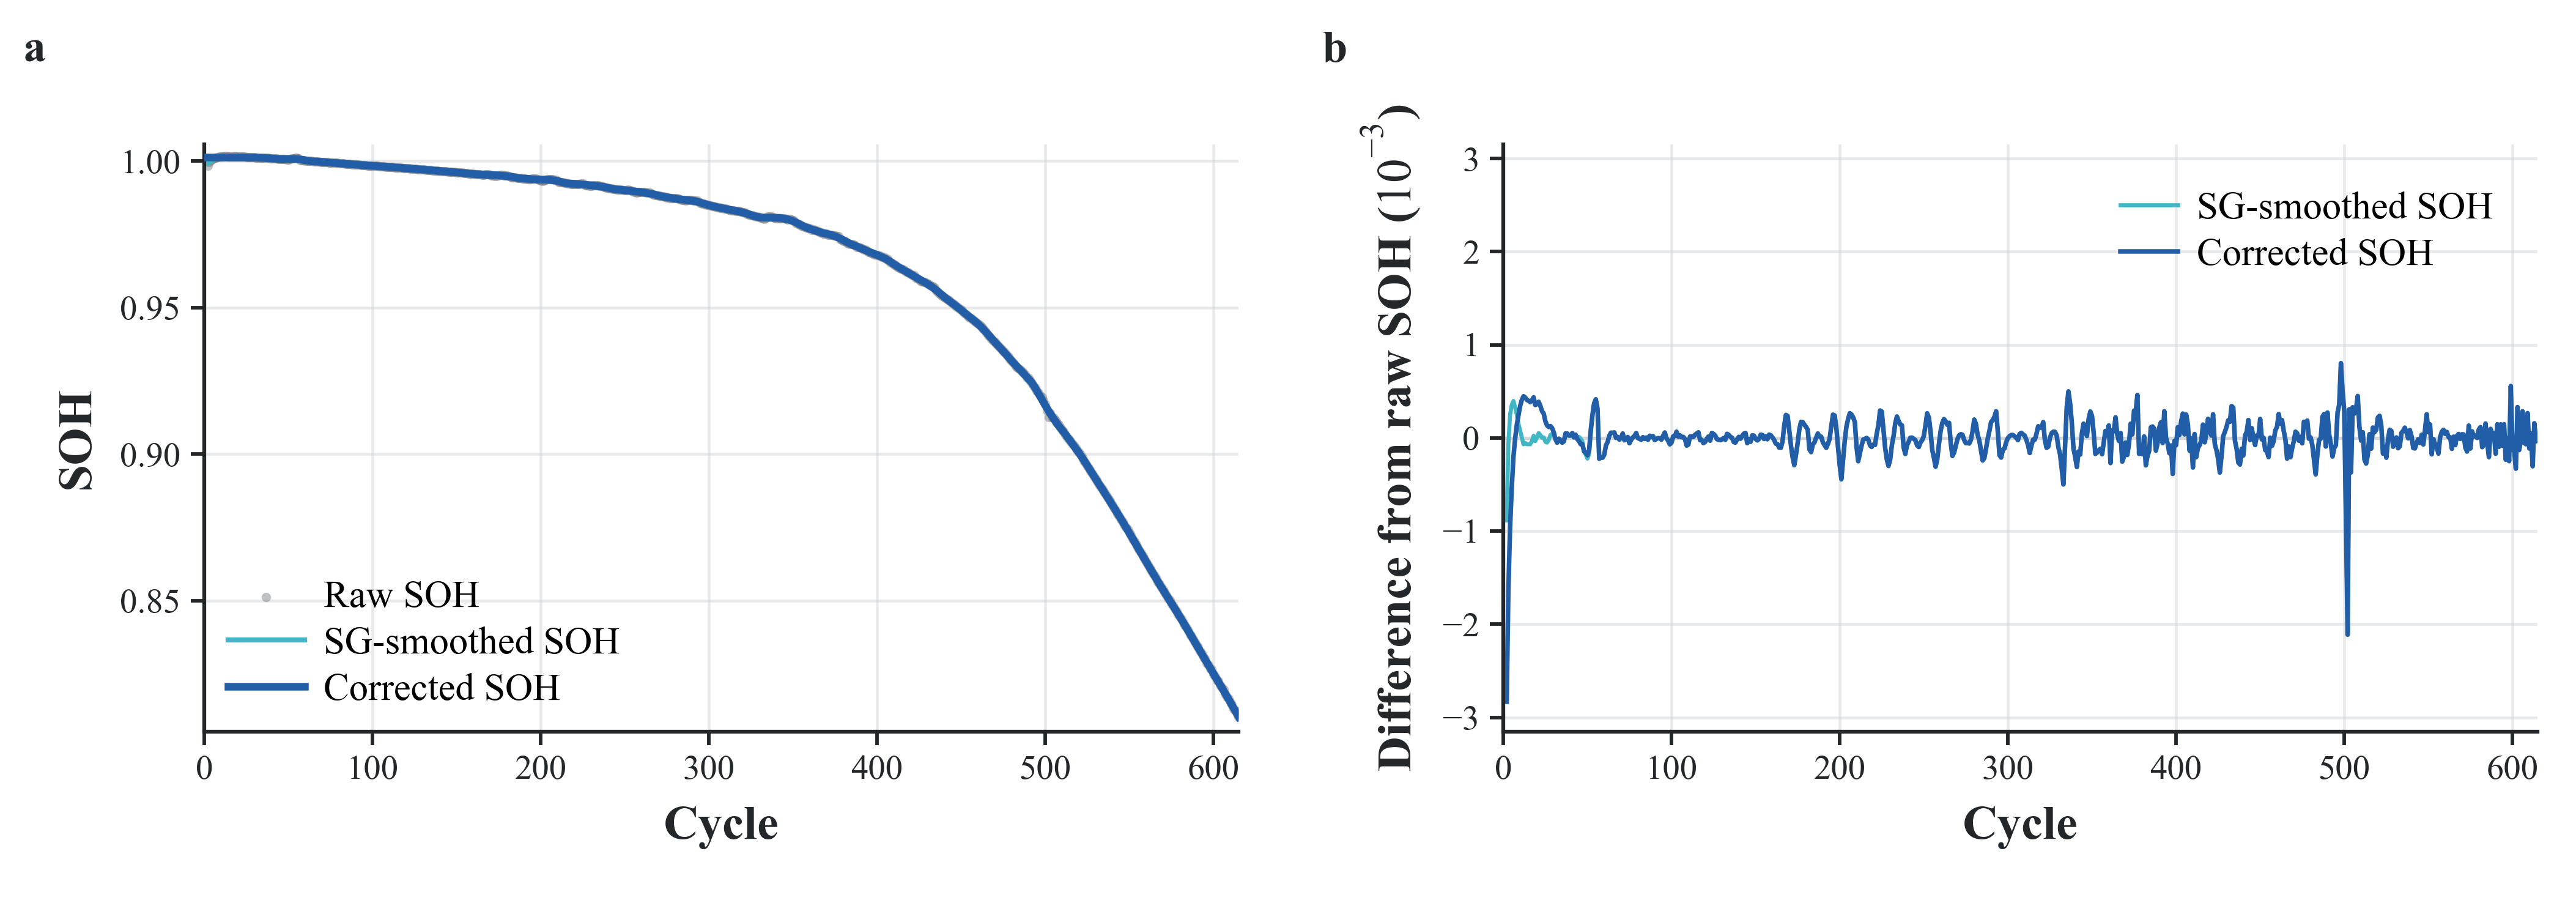
\includegraphics[width=\textwidth]{Figure1.png}
\caption{SOH preprocessing for a representative development cell. (a) SOH trajectories before and after smoothing and monotonicity correction. (b) Pointwise differences between the raw SOH record and the SG-smoothed and monotonicity-corrected trajectories.}
\label{fig:soh_preprocessing}
\end{figure}

\FloatBarrier

Figure~\ref{fig:soh_preprocessing} shows that smoothing suppresses short-scale fluctuations while retaining the overall degradation profile, whereas monotonicity correction enforces a non-increasing processed SOH trajectory. The departure panel makes the magnitude and location of these preprocessing adjustments explicit for the representative cell. Together, these steps provide a stable full-life trajectory for offline knee-label construction. The processed full-life trajectory is not used as a predictor input, and the predictor uses only measurements from cycles 1--150.

\subsection{Knee-Label Construction}\label{subsec:knee_label}

The knee cycle $y_i$ was defined from the corrected SOH trajectory using a two-segment least-squares model fitted against physical cycle number. Candidate split positions were limited to 20--90\% of the valid trajectory and required at least 30 observations on each side. Writing $\widetilde{s}_{i,r}=\widetilde{s}_i(c_{i,r})$, separate linear models were fitted before and after every admissible observation position $\ell\in\mathcal{L}_i$, and the split with the minimum total residual sum of squares was selected:
\begin{equation}
\begin{aligned}
\ell_i^*=\arg\min_{\ell\in\mathcal{L}_i}\Bigg\{&
\sum_{r\leq\ell}\left[\widetilde{s}_{i,r}-a_{i,1}(\ell)c_{i,r}-b_{i,1}(\ell)\right]^2\\
&+\sum_{r>\ell}\left[\widetilde{s}_{i,r}-a_{i,2}(\ell)c_{i,r}-b_{i,2}(\ell)\right]^2
\Bigg\},\\
y_i&=c_{i,\ell_i^*}.
\end{aligned}
\end{equation}

The target was the observed cycle with the minimum two-segment residual sum of squares. The split observation was assigned to the first segment, and the two segments were fitted independently.

To assess dependence on the label definition, two deterministic alternatives were retained as sensitivity targets. The chord-distance label characterizes the knee as the largest geometric departure from the overall degradation trend. Physical cycle and corrected SOH were normalized to $[0,1]$, and a straight chord was drawn between the trajectory endpoints. The admissible observation with the maximum perpendicular distance from this chord was selected as the knee.

The degradation-rate-threshold label instead identifies the onset of a sustained increase in capacity-fade rate. The negative numerical gradient of the corrected SOH trajectory was smoothed with an odd moving-average window of $\max(9,\operatorname{round}_{\mathrm{odd}}(0.035n_i^{\mathrm{life}}))$ observations. Let $m_i$ denote the median smoothed rate before the lower admissible boundary and let $q_{0.90,i}$ denote the 90th percentile within the admissible interval. The cell-specific threshold was
\begin{equation}
\tau_i=m_i+0.40\max\!\left(0,q_{0.90,i}-m_i\right).
\end{equation}
The first admissible observation reaching $\tau_i$ was selected as the knee; if no crossing occurred, the admissible observation with the maximum smoothed rate was used. Both alternatives were constructed offline from the corrected full-life SOH trajectory and did not change the early-cycle predictor inputs.

% \begin{figure}[t]
% \centering
% \begin{minipage}[t]{0.48\textwidth}
%   \vspace{0pt}\centering
% \includegraphics[width=\linewidth]{Figure2a.png}
% \end{minipage}\hfill%
% \begin{minipage}[t]{0.48\textwidth}
%   \vspace{0pt}\centering
% \includegraphics[width=\linewidth]{Figure2b.png}
% \end{minipage}

% \vspace{0.35em}

% \begin{minipage}[t]{0.48\textwidth}
%   \vspace{0pt}\centering
% \includegraphics[width=\linewidth]{Figure2c.png}
% \end{minipage}\hfill%
% \begin{minipage}[t]{0.48\textwidth}
%   \vspace{0pt}\centering
% \includegraphics[width=\linewidth]{Figure2d.png}
% \end{minipage}

% \vspace{0.35em}

% \begin{minipage}[t]{0.48\textwidth}
%   \vspace{0pt}\centering
% \includegraphics[width=\linewidth]{Figure2e.png}
% \end{minipage}\hfill%
% \begin{minipage}[t]{0.48\textwidth}
%   \vspace{0pt}\centering
% \includegraphics[width=\linewidth]{Figure2f.png}
% \end{minipage}
% \caption{Offline knee-label constructions for a representative development cell: (a) admissible split objective for the primary piecewise-linear label; (b) selected minimum-residual label; (c) admissible chord-distance objective; (d) normalized chord-distance geometry; (e) smoothed degradation rate, threshold, and first admissible crossing; and (f) the corresponding degradation-rate-threshold label on the corrected SOH trajectory.}
% \label{fig:piecewise_knee_label}
% \end{figure}

\begin{figure}[t]
\centering
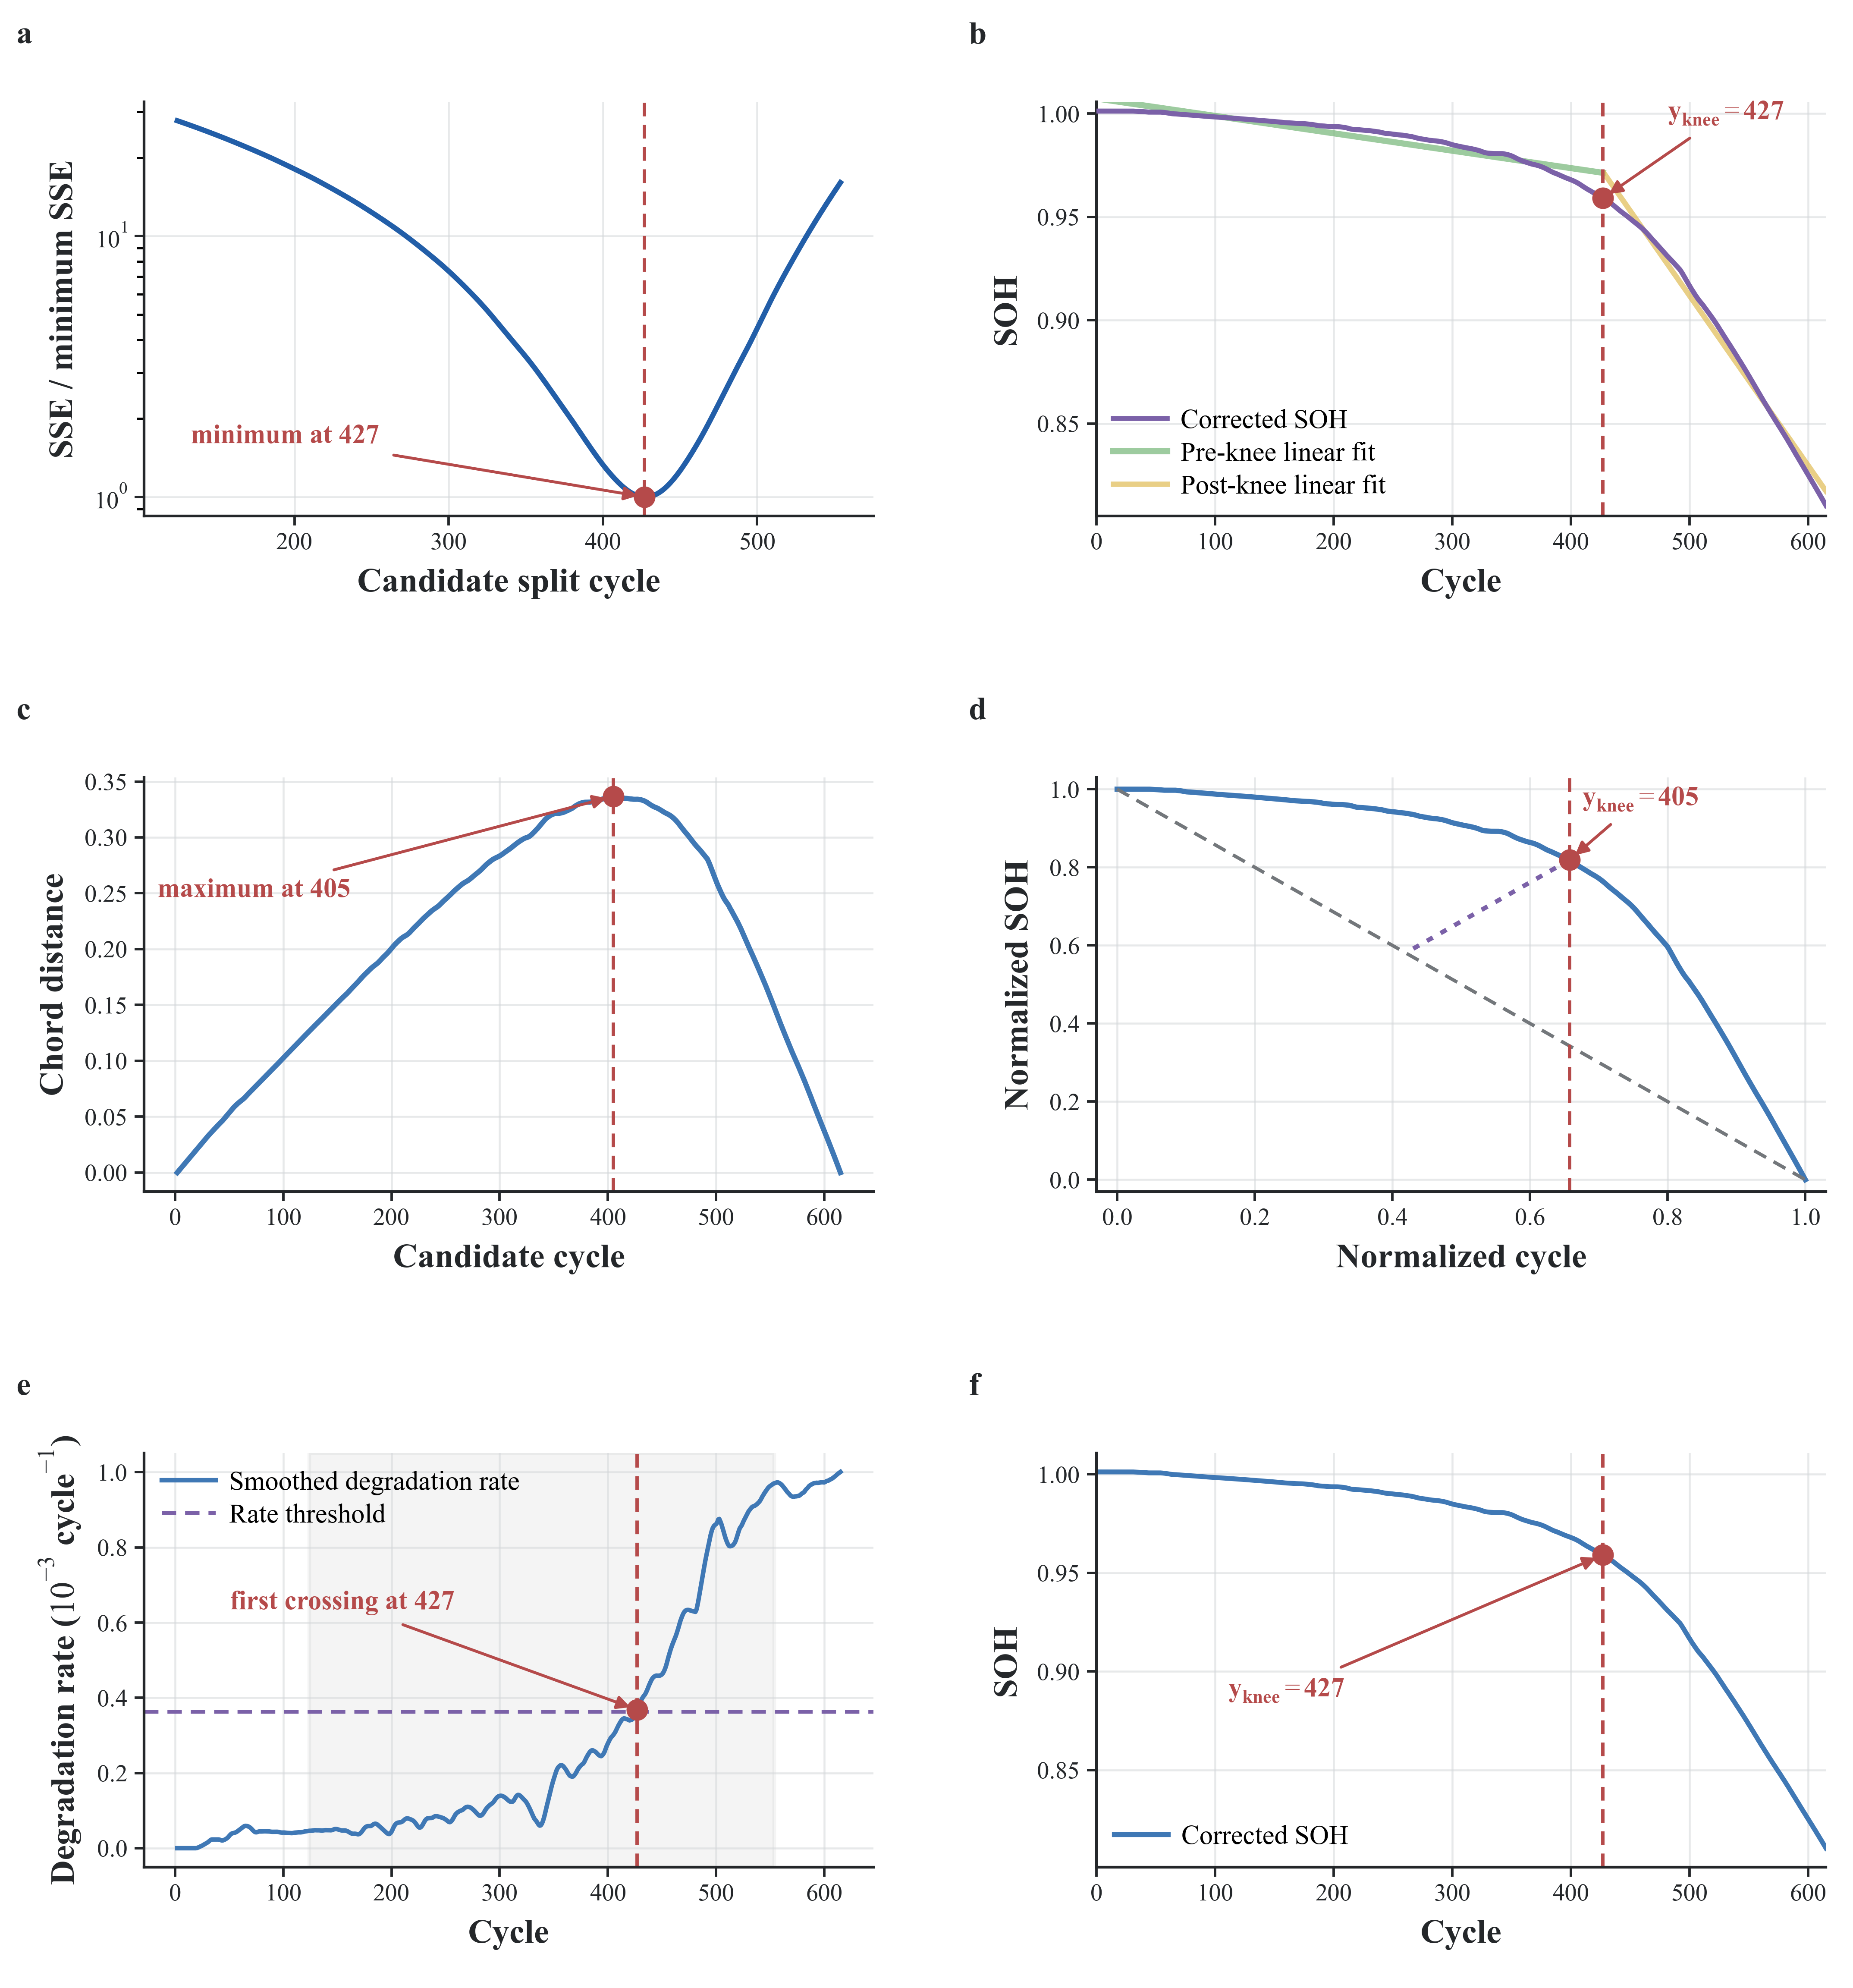
\includegraphics[width=\textwidth]{Figure2.png}
\caption{Offline knee-label constructions for a representative development cell: (a) admissible split objective for the primary piecewise-linear label; (b) selected minimum-residual label; (c) admissible chord-distance objective; (d) normalized chord-distance geometry; (e) smoothed degradation rate, threshold, and first admissible crossing; and (f) the corresponding degradation-rate-threshold label on the corrected SOH trajectory.}
\label{fig:piecewise_knee_label}
\end{figure}

\FloatBarrier

Figure~\ref{fig:piecewise_knee_label} illustrates the three offline knee-label constructions for the same representative development cell. Panels (a) and (b) present the primary piecewise-linear construction. The fitting objective reaches a pronounced minimum at cycle 427, and the corresponding two-segment fit separates the gradual pre-knee decline from the subsequent accelerated degradation, yielding the primary label $y_i=427$. Panels (c) and (d) show that the chord-distance criterion reaches its maximum at cycle 405. By emphasizing the largest geometric departure from the chord connecting the trajectory endpoints, this criterion places the knee 22 cycles earlier. Panels (e) and (f) show that the degradation-rate threshold is first crossed at cycle 427, coinciding with the primary label for this cell. 

The three constructions therefore characterize related but distinct aspects of the degradation trajectory. The piecewise-linear minimum-residual rule was adopted as the primary label because it directly compares the degradation regimes before and after each admissible split on the physical-cycle scale. The other two definitions were retained as complementary sensitivity targets, and their cohort-level agreement and predictor-level effects are evaluated in Section~4.6.

\subsection{Localized DeltaQ Representations}
\label{subsec:local_deltaq}

\begingroup
\setlength{\abovedisplayskip}{7pt plus 2pt minus 2pt}
\setlength{\belowdisplayskip}{7pt plus 2pt minus 2pt}
\setlength{\abovedisplayshortskip}{5pt plus 2pt minus 1pt}
\setlength{\belowdisplayshortskip}{5pt plus 2pt minus 1pt}

we next constructed early-cycle representations exclusively from measurements available within the first $N=150$ cycles. The cycle-10-to-150 discharge-curve difference was used to construct overlapping local-region and morphology representations that retained the positional distribution of early curve changes.

\noindent\textit{Early-cycle difference response.}
Early capacity loss can remain small after the shape of the discharge response begins to change. The public dataset provides each linearly interpolated discharge-capacity curve $Q_{d,\mathrm{lin}}$ on the same descending voltage
grid,
\begin{equation}
v_r
=
3.5-\frac{1.5r}{L-1}\ \mathrm{V},
\qquad
r=0,\ldots,L-1,
\qquad
L=1000.
\end{equation}

For convenient normalized positional indexing, we define the discharge-position coordinate
\begin{equation}
u_r
=
\frac{3.5-v_r}{1.5}
=
\frac{r}{L-1}
\in[0,1],
\end{equation}
so that $u=0$ and $u=1$ correspond to 3.5 and 2.0~V, respectively. Let $q_i^{(c)}(u_r)$ denote the $Q_{d,\mathrm{lin}}$ curve at physical cycle $c$ for cell $i$, where physical cycle $c$ corresponds to zero-based
array index $c-1$. The early-cycle difference response was defined as
\begin{equation}
\Delta q_i(u_r)
=
q_i^{(150)}(u_r)-q_i^{(10)}(u_r),
\qquad
r=0,\ldots,L-1.
\end{equation}

Cycle 10 was selected as the reference following Severson et al.~\cite{severson2019data}, whereas cycle 150 marked the end of the prescribed observation window. These two cycles were used consistently throughout the model comparisons. Because all $Q_{d,\mathrm{lin}}$ inputs shared the same 1000-point voltage grid, the curves were differenced pointwise. The coordinate $u_r$ re-indexes this grid without resampling the curves.

\noindent\textit{Local-region descriptors.}
Local DeltaQ retained positional structure along the discharge coordinate by partitioning the difference response into overlapping regions of width $W=50$ grid points and stride $H=25$,
\begin{equation}
\begin{aligned}
\Omega_m
&=
\left\{
u_{(m-1)H},
\ldots,
u_{(m-1)H+W-1}
\right\},
&&
m=1,\ldots,M,\\
M
&=
1+\left\lfloor\frac{L-W}{H}\right\rfloor
=
39.
\end{aligned}
\end{equation}

The 50\% overlap allows a localized change near one region boundary to remain represented in the neighboring region. For each $\Omega_m$, eight descriptors were calculated,
\begin{equation}
\boldsymbol{\phi}_{i,m}
=
\left[
\mu_{i,m},
s_{i,m},
\mu^{\mathrm{abs}}_{i,m},
\Delta q^{\min}_{i,m},
\Delta q^{\max}_{i,m},
R_{i,m},
\beta_{i,m},
E_{i,m}
\right],
\end{equation}
where the entries denote the local mean, sample standard deviation, mean absolute response, minimum, maximum, range, least-squares slope, and energy, respectively. The energy descriptor was defined as
\begin{equation}
E_{i,m}
=
\frac{1}{W}
\sum_{u_r\in\Omega_m}
\Delta q_i(u_r)^2.
\end{equation}
These descriptors formed the prespecified local candidate dictionary.

\noindent\textit{Morphology descriptors.}
The 39 local regions yielded $39\times8=312$ descriptors. Fourteen additional matrix-profile-inspired descriptors summarized recurrent and atypical shapes from 50-point subsequences extracted with a stride of 10 \cite{yeh2016matrix}. Together, the 312 local-region descriptors and 14 morphology descriptors formed a 326-dimensional localized DeltaQ candidate pool.

\endgroup


\subsection{Feature Dictionary}
\label{subsec:feature_assembly}

The fixed feature block comprised 30 descriptors: 22 calculated from valid discharge-capacity and raw-SOH observations within the first 150 cycles, and eight Global DeltaQ whole-curve statistics calculated from the cycle-150 minus cycle-10 difference response.

For cell $i$, let
\[
\mathcal{V}_i
=
\left(
t_{i,1},
\ldots,
t_{i,n_i^{(150)}}
\right)
\]
denote the ordered sequence of physical cycle numbers satisfying $t_{i,\ell}\leq150$ for which $Q_{i,t_{i,\ell}}^{\mathrm d}$ is finite and positive. Define
\[
q_{i,\ell}
=
Q_{i,t_{i,\ell}}^{\mathrm d},
\qquad
s_{i,\ell}
=
s_i^{\mathrm{raw}}(t_{i,\ell}).
\]

The sample standard deviation was calculated using the $n_i^{(150)}-1$ denominator. For $x\in\{q,s\}$, the first-to-last change was defined as
\[
\Delta x_i
=
x_{i,n_i^{(150)}}-x_{i,1}.
\]
The raw-SOH slope and intercept were obtained by ordinary least-squares regression against physical cycle number.

For the positive-increment descriptors, let
\[
d_{i,\ell}
=
s_{i,\ell+1}-s_{i,\ell},
\qquad
\ell=1,\ldots,n_i^{(150)}-1,
\]
and set $\delta=10^{-4}$. The number, cumulative amplitude, and maximum amplitude of positive increments were defined as
\[
\sum_{\ell=1}^{n_i^{(150)}-1}
\mathbb{I}(d_{i,\ell}>\delta),
\qquad
\sum_{\ell:d_{i,\ell}>\delta}d_{i,\ell},
\]
and
\[
\max\left(
\{d_{i,\ell}:d_{i,\ell}>\delta\}
\cup
\{0\}
\right),
\]
respectively. The tolerance $\delta=10^{-4}$ corresponds to 0.01 percentage points of SOH.

The eight Global DeltaQ descriptors were calculated over the complete cycle-150 minus cycle-10 difference response $\Delta q_i(u_r)$. They comprised the mean, sample standard deviation, minimum, maximum, range, mean absolute response, skewness, and kurtosis. The capacity/SOH descriptors were derived from valid observations at $t\leq150$, whereas the Global DeltaQ descriptors summarized the complete difference response. The resulting 30 fixed descriptors are listed in Table~\ref{tab:fixed_feature_definitions}.

\begin{table}[!htbp]
\centering
\caption{Grouped definitions of the 30 fixed early-cycle descriptors.}
\label{tab:fixed_feature_definitions}
\small
\renewcommand{\arraystretch}{1.08}
\setlength{\tabcolsep}{5pt}

\begin{tabularx}{\textwidth}{
@{}
>{\centering\arraybackslash}m{0.20\textwidth}
>{\raggedright\arraybackslash}X
@{}
}
\toprule
\textbf{Group (count)} & \textbf{Included descriptors} \\
\midrule

Availability (1) & Number of valid observations, $n_i^{(150)}=|\mathcal{V}_i|$.
\\[4pt]

Capacity (9) & Mean, sample standard deviation, minimum, maximum, first value, last value, range, last--first change, and last/first ratio.
\\[4pt]

Raw SOH (9) & Mean, sample standard deviation, minimum, maximum, first value, last value, last--first change, and OLS slope and intercept.
\\[4pt]

Positive increments (3) & Number, cumulative amplitude, and maximum amplitude of increases between adjacent valid SOH observations exceeding $\delta=10^{-4}$.
\\[4pt]

Global DeltaQ (8) & Mean, sample standard deviation, minimum, maximum, range, mean absolute response, skewness, and kurtosis of the cycle-150 minus cycle-10 difference response.
\\

\bottomrule
\end{tabularx}
\end{table}

The complete unfiltered feature dictionary therefore comprised 30 fixed descriptors and 326 localized DeltaQ candidates:
\begin{equation}
\mathbf{z}_i
=
\left[
\mathbf{z}_i^{\mathrm{fixed}},
\boldsymbol{\Phi}_i^{\mathrm{local/morph}}
\right]
\in\mathbb{R}^{356},
\end{equation}
where
\[
\mathbf{z}_i^{\mathrm{fixed}}
=
\left[
\mathbf{z}_i^{\mathrm{raw/SOH}},
\mathbf{z}_i^{\mathrm{global}\,\Delta Q}
\right]
\in\mathbb{R}^{30},
\]
and $\boldsymbol{\Phi}_i^{\mathrm{local/morph}}\in\mathbb{R}^{326}$ collects the local-region and morphology descriptors.

The 30 fixed descriptors were retained without supervised feature selection, whereas the 326 localized DeltaQ candidates were subjected to training-fold eligibility screening and supervised selection before model fitting, as specified in Section~\ref{sec:model}.

% Section 3: model

\FloatBarrier
\section{Methodology}
\label{sec:model}

Building on the feature representations defined in Section~2, the proposed stability-aware Local DeltaQ--ExtraTrees framework (LDQ-ET) maps early-cycle measurements to absolute knee-cycle estimates while using the full-life SOH trajectory only for offline label construction. Figure~\ref{fig:methodology_framework} summarizes the three-stage workflow: Panel (a) separates the early predictor inputs from the offline target, Panel (b) confines feature selection and ExtraTrees development to the training data, and Panel (c) applies the frozen pipeline to the held-out primary and secondary cohorts. The corresponding feature-selection, model-fitting, and evaluation procedures are detailed in Sections~3.1--3.3.

\begin{figure}[t]
\centering
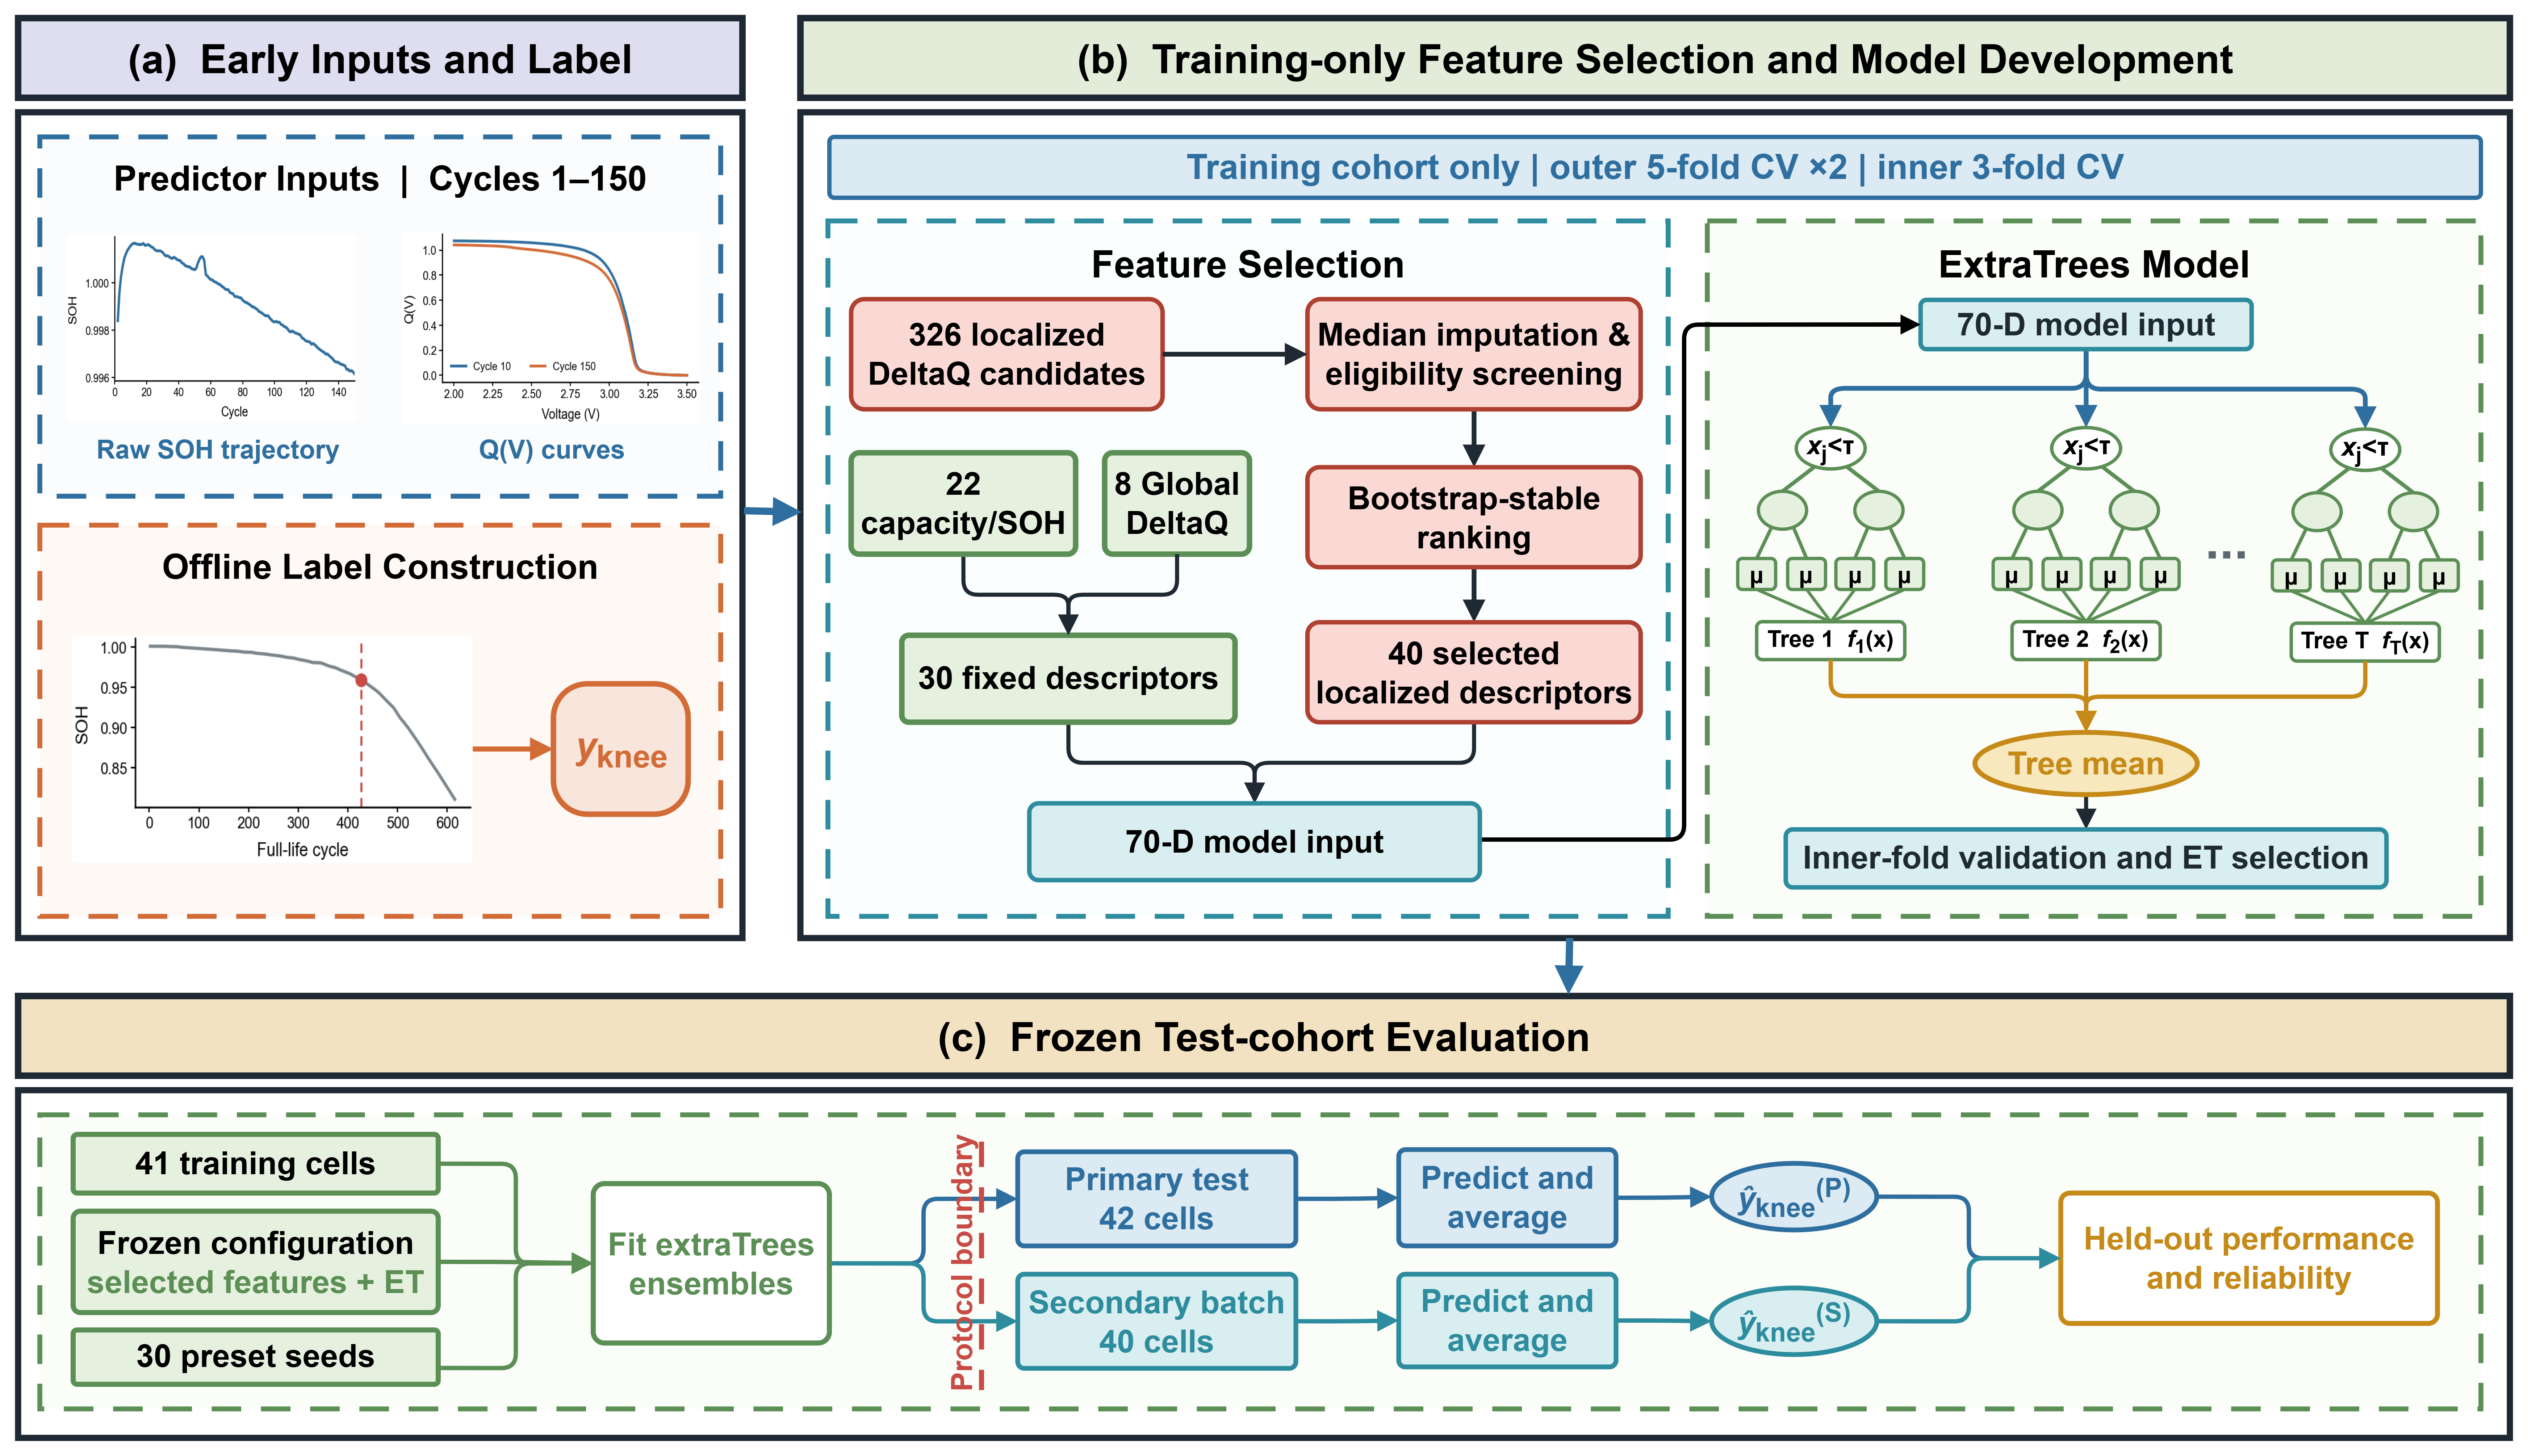
\includegraphics[page=1,width=\linewidth]{Figure3.png}
\caption{Overview of the LDQ-ET framework and held-out evaluation workflow.}
\label{fig:methodology_framework}
\end{figure}

\subsection{DeltaQ-Derived Descriptor Selection}
\label{subsec:region_selection}

The 326 local DeltaQ-derived candidates comprised 312 local-region descriptors and 14 morphology descriptors. To obtain a compact representation under a common feature budget, each selector retained $K=40$ descriptors from this candidate pool. Five selector families were then evaluated, emphasizing univariate relevance (Pearson), resampling stability (Bootstrap-stable), regional coverage (Region-balanced), contiguous structure (Contiguous-band), and relevance--redundancy trade-offs (mRMR-style). All imputation \cite{wilimitis2023crossvalidation}, scoring, and selection statistics were estimated exclusively from the training portion of each nested-development split \cite{ambroise2002selectionbias, varma2006crossvalidation, krstajic2014pitfalls}.

For a training set $\mathcal{D}$, non-finite entries are imputed with the corresponding training-partition median, and zero-variance candidates are excluded before scoring. Candidate relevance is measured by the absolute Pearson correlation with the knee cycle,
\begin{equation}
\rho_j(\mathcal{D})=
\left|\frac{\sum_{i\in\mathcal{D}}(\Phi_{ij}-\bar{\Phi}_j)(y_i-\bar{y})}
{\sqrt{\sum_{i\in\mathcal{D}}(\Phi_{ij}-\bar{\Phi}_j)^2}
\sqrt{\sum_{i\in\mathcal{D}}(y_i-\bar{y})^2}}\right|.
\end{equation}

Absolute Pearson correlation was used as the univariate relevance score. The Pearson selector ranked the eligible candidates by $\rho_j(\mathcal{D})$ and retained the 40 highest-ranked descriptors.

From $\mathcal{D}$, $B$ cell-level bootstrap samples are drawn following the principle of resampling-stability selection \cite{meinshausen2010stability}. Let $I_j^{(b)}=1$ when candidate $j$ belongs to the top-$K$ ranking in bootstrap sample $b$, and let $I_j^{(b)}=0$ otherwise. Its selection frequency and mean bootstrap relevance are
\begin{equation}
\pi_j=\frac{1}{B}\sum_{b=1}^{B}I_j^{(b)},
\qquad
\bar{\rho}_j=\frac{1}{B}\sum_{b=1}^{B}\rho_j^{(b)}.
\end{equation}
A stability-aware score combines reproducible top-$K$ membership with normalized association strength,
\begin{equation}
z_j=\pi_j+0.25
\frac{\bar{\rho}_j}
{\max\!\left(\max_{\ell}\bar{\rho}_{\ell},\varepsilon\right)},
\end{equation}
where $\varepsilon=10^{-12}$ prevents a zero denominator. The frequency term favors associations that recur across bootstrap samples, whereas the normalized relevance term preserves information about association strength. The Bootstrap-stable selector ranks eligible candidates by $z_j$ and retains the top 40. The number of bootstrap samples was fixed at $B=40$.

The Region-balanced selector limits the same $z_j$ ranking to $c=2$ descriptors per ordered region, with morphology descriptors treated as a separate group. The Contiguous-band selector takes the maximum $z_j$ per region, applies adjacent-region weights of 0.25, 0.50, and 0.25, and identifies the best seven-region band. It selects 32 descriptors from that band and eight from its complement. The correlation-based mRMR-style selector starts from the most relevant candidate. At each subsequent step, it maximizes Pearson relevance minus 0.15 times the candidate's mean absolute correlation with the current selected set \cite{peng2005feature}. Together, the five selectors provide matched controls for relevance, stability, spatial distribution, contiguity, and redundancy. Their scores quantify predictive association rather than evidence for a unique electrochemical mechanism.

For selector-family finalization, each family $m$ was ranked using the training-only development score
\begin{equation}
S_m=\overline{\mathrm{MAE}}_m+0.10\,s_m+0.10\,\mathrm{MAE}^{\max}_m,
\label{eq:selector_development_score}
\end{equation}
where $\overline{\mathrm{MAE}}_m$, $s_m$, and $\mathrm{MAE}^{\max}_m$ are the mean, standard deviation, and maximum MAE across repeated outer folds, respectively. Lower values were preferred. This score was used only to rank selector families within the training cohort; held-out cohorts did not contribute to selector finalization. The selector family with the lowest development score, $m^{*}=\arg\min_m S_m$, was retained for final refitting.

\subsection{ExtraTrees Prediction And Pipeline Finalization}\label{subsec:ldqet_prediction}

For cell $i$, the selector returns $\mathcal{S}_{\mathcal{D}}=\mathcal{A}(\mathcal{D})$. The 30-dimensional always-retained vector $\mathbf{z}_i^{\mathrm{fixed}}$ comprises the 22 raw capacity/SOH descriptors and eight Global DeltaQ descriptors. It is concatenated with the selected DeltaQ-derived descriptors,
\begin{equation}
\mathbf{x}_i =
\left[\mathbf{z}_i^{\mathrm{fixed}},
\boldsymbol{\Phi}_{i,\mathcal{S}_{\mathcal{D}}}\right].
\end{equation}
With 40 selected DeltaQ-derived descriptors and 30 fixed descriptors, $\mathbf{x}_i\in\mathbb{R}^{70}$. This vector is mapped to an absolute knee-cycle estimate using an Extremely Randomized Trees regressor \cite{geurts2006extremely}. For an ensemble of $T$ randomized regression trees,
\begin{equation}
\hat{y}_i = \frac{1}{T}\sum_{t=1}^{T} h_t(\mathbf{x}_i),
\end{equation}
where $h_t(\cdot)$ denotes the $t$th tree. The same 70-dimensional vector is supplied to every tree. At each node, ExtraTrees evaluates randomized thresholds over a random 50\% feature subset and retains the split that produces the largest reduction in regression impurity. Each terminal leaf returns the mean training target of the samples assigned to that leaf, and the final prediction averages the tree outputs. This construction represents nonlinear interactions without requiring feature scaling or a prescribed parametric relation to the knee cycle.

All fitted quantities are training-fold specific during nested development. These include imputation medians, selector scores, the selected descriptors, the selected ExtraTrees hyperparameters, and the fitted tree structures. Nested development selected a minimum leaf size of 1, using 500 trees for model screening. Under a prespecified tree-count policy, this selected structural configuration was then refitted with 1200 trees for each final ensemble. The increase in tree count was applied only after configuration selection and did not constitute further hyperparameter optimization. 

The selector family retained during nested development was then refitted once on all 41 training cells to obtain the frozen 40-feature subset. Thirty ExtraTrees ensembles were fitted to the same imputed 70-dimensional training matrix using the prespecified seeds 123--152. For test cell $i$, the reported point estimate is
\begin{equation}
\overline{y}_i=
\frac{1}{30}\sum_{s=123}^{152}\widehat{y}_i^{(s)},
\end{equation}
where $\widehat{y}_i^{(s)}$ is the prediction from the ensemble fitted with seed $s$. Only the ExtraTrees randomization varied across the 30 fits; the selected feature subset and imputation statistics remained fixed.

\subsection{Performance Metrics and Empirical Reliability Assessment}
\label{subsec:reliability_protocol}

Predictive performance is assessed at the cell level using mean absolute error (MAE), root mean squared error (RMSE), the coefficient of determination ($R^2$), and the 90th percentile of absolute error
(q90-AE). These metrics summarize the typical error magnitude, place greater weight on larger errors, measure performance relative to the mean-target baseline, and characterize the upper tail of the absolute-error distribution, respectively. For $n$ evaluated cells, MAE and RMSE are defined as
\begin{equation}
\mathrm{MAE}=
\frac{1}{n}\sum_{i=1}^{n}\left|y_i-\overline{y}_i\right|,
\label{eq:mae}
\end{equation}
\begin{equation}
\mathrm{RMSE}=
\sqrt{\frac{1}{n}\sum_{i=1}^{n}\left(y_i-\overline{y}_i\right)^2},
\label{eq:rmse}
\end{equation}
where $\overline{y}_i$ is the 30-seed mean prediction defined in Section~\ref{subsec:ldqet_prediction}. The coefficient of determination is
\begin{equation}
R^2=
1-\frac{\sum_{i=1}^{n}\left(y_i-\overline{y}_i\right)^2}
{\sum_{i=1}^{n}\left(y_i-\bar{y}\right)^2},
\qquad
\bar{y}=\frac{1}{n}\sum_{i=1}^{n}y_i.
\label{eq:r2}
\end{equation}
MAE and RMSE are reported in cycles, whereas $R^2$ is dimensionless. The q90 absolute error, which is also reported in cycles, is defined as
\begin{equation}
q_{0.90}^{\mathrm{AE}}=
Q_{0.90}\!\left(
\left\{|y_i-\overline{y}_i|\right\}_{i=1}^{n}
\right),
\end{equation}

Reliability is further assessed from the complete cell-level error distribution and a training-calibrated empirical interval. To calibrate the interval without using the held-out cohorts, out-of-fold predictions were obtained for the training cells during the repeated outer-CV procedure. Each training cell received one out-of-fold prediction in each of the two outer-CV repeats. Let $\widehat{y}_{i,a}^{\mathrm{OOF}}$ denote the prediction for cell $i$ from repeat $a\in\{1,2\}$. The repeat-averaged out-of-fold prediction and the corresponding absolute calibration residual were defined as
\begin{equation}
\widehat{y}_i^{\mathrm{OOF}}
=
\frac{1}{2}
\sum_{a=1}^{2}
\widehat{y}_{i,a}^{\mathrm{OOF}},
\qquad
e_i^{\mathrm{OOF}}
=
\left|
y_i-\widehat{y}_i^{\mathrm{OOF}}
\right|.
\label{eq:oof_residual}
\end{equation}

For $n_{\mathrm{cal}}=41$ training cells, the empirical interval half-width associated with the target level $1-\alpha$ was defined as
\begin{equation}
r_{\alpha}=Q_{\lceil(n_{\mathrm{cal}}+1)(1-\alpha)\rceil/n_{\mathrm{cal}}}
\left(\left\{e_i^{\mathrm{OOF}}\right\}_{i=1}^{n_{\mathrm{cal}}}\right),
\end{equation}
where $Q$ is the empirical quantile evaluated using the \texttt{higher} empirical-quantile rule. For the test-cell point estimate $\overline{y}_i$ defined above, the interval is
\begin{equation}
\mathcal{I}_i(\alpha)=
\left[\overline{y}_i-r_{\alpha},\overline{y}_i+r_{\alpha}\right].
\end{equation}
We used $\alpha=0.10$. The resulting constant-width interval was used to summarize empirical uncertainty around each point estimate and to compare coverage behavior between the primary and secondary cohorts.

\FloatBarrier
\section{Experimental Results and Analysis}\label{sec:results}

\subsection{Evaluation Cohorts}
\label{subsec:experimental_design}

The official partitions defined by Severson et al.~\cite{severson2019data} were retained as the basis of the evaluation design. After offline knee-label construction (Section~\ref{subsec:knee_label}), one primary-test cell (\texttt{b2c1}, $y_i=94$) was excluded because its knee occurred within the 150-cycle observation window and did not satisfy the prespecified requirement $y_i>150$. The final evaluation cohorts comprised 41 training cells, 42 primary-test cells, and 40 secondary-test cells. Table~\ref{tab:dataset} summarizes their sizes and knee-cycle distributions, with knee cycles reported as the median and the first and third quartiles in brackets.

\begin{table}[!ht]
\caption{Cell counts and knee-cycle distributions across the evaluation cohorts.}
\label{tab:dataset}
\centering
\fontsize{8.5pt}{10.2pt}\selectfont
\setlength{\tabcolsep}{6pt}
\renewcommand{\arraystretch}{1.12}

\begin{tabular}{@{}
>{\centering\arraybackslash}m{0.33\textwidth}
>{\centering\arraybackslash}m{0.20\textwidth}
>{\centering\arraybackslash}m{0.43\textwidth}
@{}}
\toprule
Cohort &
Cells count &
Knee cycle, median [$Q_1$, $Q_3$] \\
\midrule
Train & 41 & 428 [377, 580] \\
Primary test & 42 & 429.5 [385.25, 629.5] \\
Secondary test & 40 & 796.5 [670.25, 905] \\
\bottomrule
\end{tabular}
\end{table}
\FloatBarrier

The 41-cell training cohort was used for nested model development and pipeline finalization. The frozen pipeline was then applied without modification to the primary-test and secondary-test cohorts, which assessed same-batch performance and performance under the observed batch shift, respectively. 

The training and primary-test cohorts showed nearly identical median knee cycles of 428 and 429.5, together with substantially overlapping interquartile ranges, indicating broadly comparable target distributions. In contrast, the secondary-test cohort had a median knee cycle of 796.5, approximately 369 cycles later than that of the training cohort. Its interquartile range of $[670.25,905]$ also lay entirely above those of the training and primary-test cohorts. The secondary-test evaluation therefore examined the frozen pipeline under a pronounced shift toward later degradation transitions, rather than on another cohort with a target distribution similar to that used for model development.

\subsection{Selector Comparison And Final Representation}
\label{subsec:main_results}

The 326 localized DeltaQ candidates provide overlapping and potentially redundant descriptions of early curve changes. Relative to the 41-cell development cohort, this high-dimensional and strongly correlated candidate pool can increase estimation variance, destabilize the retained feature set, and obscure the contribution of informative discharge regions. A compact feature-selection step was therefore required before model fitting. We therefore compared the five selector families defined in Section~\ref{subsec:region_selection} in terms of predictive accuracy, cross-fold reproducibility, and spatial coverage. All selectors were evaluated using the same repeated outer 5-fold cross-validation procedure with two repeats, the same candidate pool, a fixed feature budget of $K=40$, and identical imputation and ExtraTrees development settings.

\begin{table}[!ht]
\caption{Training-only comparison of five selector families across ten repeated outer folds. MAE is reported in cycles.}
\label{tab:selector_metrics}
\centering
\small
\setlength{\tabcolsep}{2.5pt}
\renewcommand{\arraystretch}{1.12}
\begingroup
\renewcommand{\tabularxcolumn}[1]{m{#1}}
\begin{tabularx}{\textwidth}{@{}>{\raggedright\arraybackslash}m{0.22\textwidth}*{4}{>{\centering\arraybackslash}X}@{}}
\toprule
Selector & Outer-fold MAE (mean $\pm$ SD) & Worst-fold MAE & Mean Jaccard \\
\midrule
Bootstrap-stable    & $48.91\pm27.65$ & 101.28 & 0.728 \\
Contiguous-band     & $53.17\pm30.63$ & 114.23 & 0.660 \\
Region-balanced     & $52.78\pm29.31$ & 110.81 & 0.632 \\
Pearson             & $56.67\pm32.55$ & 118.86 & 0.593 \\
mRMR-style          & $54.49\pm31.98$ & 113.89 & 0.622 \\
\botrule
\end{tabularx}
\endgroup
\end{table}

\FloatBarrier

Table~\ref{tab:selector_metrics} summarizes the training-only results across ten repeated outer folds. Outer-fold MAE is reported as the mean $\pm$ standard deviation, while mean Jaccard quantifies the reproducibility of the selected feature sets across folds, with larger values indicating greater cross-fold agreement.

Across selector families, mean outer-fold MAEs ranged from 48.91 to 56.67 cycles, while worst-fold MAEs ranged from 101.28 to 118.86 cycles. Bootstrap-stable achieved the lowest mean outer-fold MAE and the lowest worst-fold MAE. It also yielded the highest mean Jaccard coefficient of 0.728, indicating greater reproducibility of the selected descriptor sets across outer folds than the other selector families.

\FloatBarrier

% \begin{figure}[t]
% \centering
% \begin{minipage}[t]{0.48\textwidth}
%   \vspace{0pt}\centering
%   \includegraphics[width=\linewidth]{Figure4a.png}
% \end{minipage}\hfill%
% \begin{minipage}[t]{0.48\textwidth}
%   \vspace{0pt}\centering
%   \includegraphics[width=\linewidth]{Figure4b.png}
% \end{minipage}

% \vspace{0.35em}

% \begin{minipage}[t]{0.48\textwidth}
%   \vspace{0pt}\centering
%   \includegraphics[width=\linewidth]{Figure4c.png}
% \end{minipage}\hfill%
% \begin{minipage}[t]{0.48\textwidth}
%   \vspace{0pt}\centering
%   \includegraphics[width=\linewidth]{Figure4d.png}
% \end{minipage}

% \caption{Training-only selector comparison at a 150-cycle observation budget. (a) Distribution of outer-fold MAE across ten repeats. (b) Mean--worst-fold error trade-off. (c) Cross-fold stability of selected feature sets, measured by pairwise Jaccard overlap. (d) Mean selected local-descriptor count along ordered discharge segments; whole-curve morphology descriptors are omitted.}
% \label{fig:selector_comparison}
% \end{figure}

\begin{figure*}[t]
  \centering
  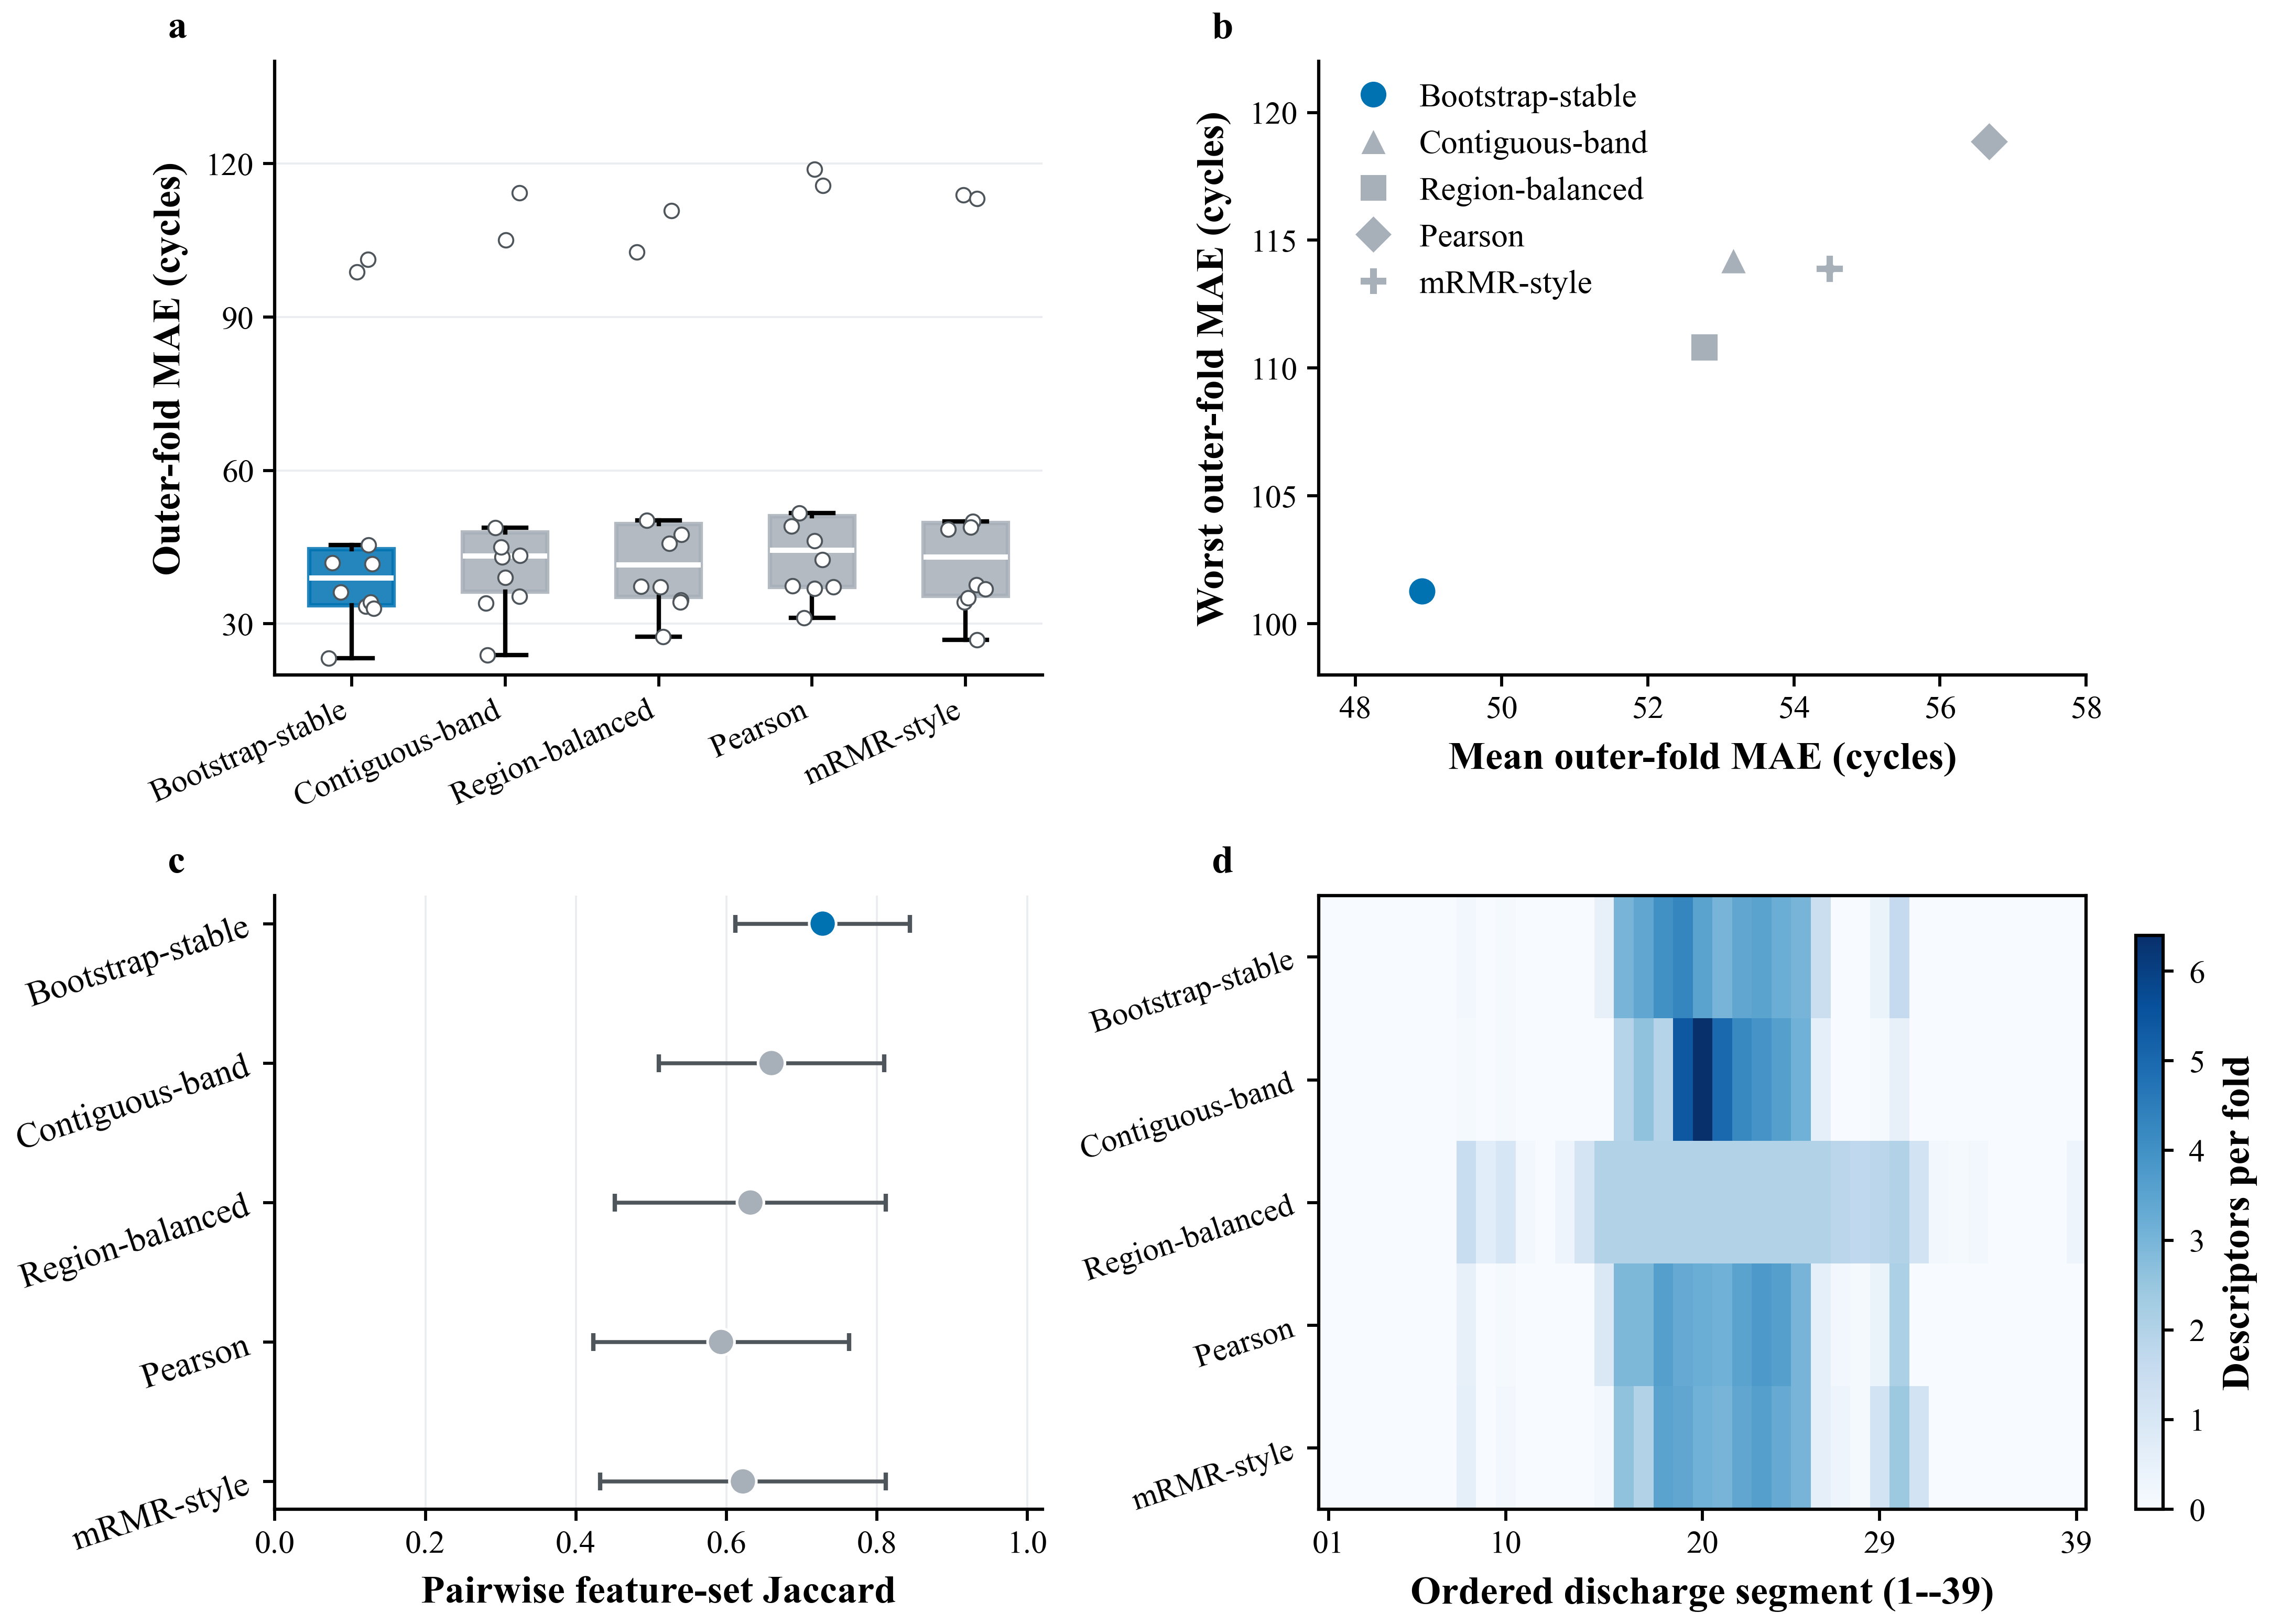
\includegraphics[width=\textwidth]{Figure4.png}
  \caption{Training-only selector comparison at a 150-cycle observation budget.}
  \label{fig:selector_comparison}
\end{figure*}

\FloatBarrier

Figure~\ref{fig:selector_comparison}a shows substantial overlap among the fold-wise MAE distributions, although Bootstrap-stable exhibits a lower central tendency than the other selector families. Figure~\ref{fig:selector_comparison}b places Bootstrap-stable at the joint minimum of mean and worst-fold MAE, visually confirming its advantages in both average predictive accuracy and worst-fold robustness. Figure~\ref{fig:selector_comparison}c further shows that Bootstrap-stable achieves the highest mean pairwise feature-set Jaccard, indicating the strongest cross-fold reproducibility of the selected descriptors.

The regional maps in Figure~\ref{fig:selector_comparison}d reveal a common emphasis on the middle portion of the discharge coordinate. Contiguous-band produces the most concentrated selection pattern, whereas Region-balanced distributes its selections over a broader range of discharge segments. By comparison, Bootstrap-stable maintains a consistent emphasis on the middle-discharge segments without concentrating excessively on a narrow region or dispersing selections too broadly, thereby providing a comparatively balanced pattern between regional concentration and spatial coverage.

Taken together, the tabulated results and visual comparisons show that Bootstrap-stable provides the most favorable combination of average predictive accuracy, worst-fold robustness, and cross-fold feature-set reproducibility. Bootstrap-stable was therefore selected as the finalized selector family for downstream modeling. Refitting it on all training cells retained 37 local-region descriptors and three morphology descriptors. Together with the 30 fixed raw/SOH and Global DeltaQ descriptors, these formed the final 70-dimensional representation used for downstream modeling.

\FloatBarrier
\subsection{Same-Batch Performance And Generalization Under Batch Shift}
\label{subsec:test_performance}

To distinguish same-batch predictive performance from generalization under batch shift, the finalized LDQ-ET model was evaluated on two held-out cohorts with different relationships to the development data. As described in Section~\ref{subsec:experimental_design}, the 42-cell primary-test cohort originated from the same batch and had a knee-cycle distribution close to that of the training cohort, whereas the 40-cell secondary-batch cohort exhibited substantially later knee cycles and provided a more demanding transfer setting.

Following the selector comparison in Section~4.2, Bootstrap-stable was fixed as the local-descriptor selector, yielding the finalized 70-dimensional LDQ-ET representation. This representation and the 1200-tree ExtraTrees regressor were then fixed under the 150-cycle observation budget and evaluated on both cohorts without further modification. Performance was summarized using cell-level MAE, RMSE, $R^2$, and the 90th-percentile absolute error (q90-AE), with 95\% confidence intervals reported in Table~\ref{tab:heldout_summary}.

\begin{table}[!ht]
\caption{Summary of test-cohort predictive performance. Values in brackets indicate 95\% confidence intervals.}
\label{tab:heldout_summary}
\centering
\footnotesize
\setlength{\tabcolsep}{1.6pt}
\renewcommand{\arraystretch}{1.50}
\begingroup
\renewcommand{\tabularxcolumn}[1]{m{#1}}
\begin{tabularx}{\textwidth}{
@{}
>{\raggedright\arraybackslash}m{0.24\textwidth}
>{\centering\arraybackslash}m{0.05\textwidth}
*{4}{>{\centering\arraybackslash}X}
@{}
}
\toprule
Test cohort 
& $n$ 
& \shortstack{MAE (cycles)\\ \mbox{[95\% CI]}} 
& \shortstack{RMSE (cycles)\\ \mbox{[95\% CI]}} 
& \shortstack{$R^2$\\ \mbox{[95\% CI]}} 
& \shortstack{q90 AE (cycles)\\ \mbox{[95\% CI]}} \\
\midrule
Primary test (same batch) 
& 42 
& \shortstack{38.23\\ \mbox{[26, 52]}} 
& \shortstack{56.87\\ \mbox{[38, 76]}} 
& \shortstack{0.957\\ \mbox{[0.895, 0.979]}} 
& \shortstack{95.50\\ \mbox{[59, 123]}} \\
Secondary test (cross-batch) 
& 40 
& \shortstack{64.15\\ \mbox{[46, 84]}} 
& \shortstack{88.74\\ \mbox{[61, 114]}} 
& \shortstack{0.868\\ \mbox{[0.778, 0.919]}} 
& \shortstack{153.15\\ \mbox{[79, 204]}} \\
\botrule
\end{tabularx}
\endgroup
\end{table}

% \begin{figure}[!ht]
% \centering
% \begin{minipage}[t]{0.48\textwidth}
%   \vspace{0pt}\centering
%   \includegraphics[width=\linewidth]{Figure5a.png}
% \end{minipage}\hfill%
% \begin{minipage}[t]{0.48\textwidth}
%   \vspace{0pt}\centering
%   \includegraphics[width=\linewidth]{Figure5b.png}
% \end{minipage}

% \vspace{0.35em}

% \begin{minipage}[t]{0.48\textwidth}
%   \vspace{0pt}\centering
%   \includegraphics[width=\linewidth]{Figure5c.png}
% \end{minipage}\hfill%
% \begin{minipage}[t]{0.48\textwidth}
%   \vspace{0pt}\centering
%   \includegraphics[width=\linewidth]{Figure5d.png}
% \end{minipage}

% \caption{Test-cohort performance of the frozen LDQ-ET pipeline. (a) Observed and predicted knee cycles. 
% (b) Absolute-error distributions. 
% (c) The 12 largest cell-level absolute errors. 
% (d) Cohort-level MAE across 30 prespecified ExtraTrees seeds; these values assess algorithmic reproducibility rather than independent experimental replication. 
% Colors distinguish the primary (blue) and secondary (orange) cohorts. 
% Cell identifiers use \texttt{bNcM}, where \texttt{bN} denotes the source batch and \texttt{cM} denotes the cell identifier.}
% \label{fig:external_prediction}
% \end{figure}

\begin{figure}[!ht] 
\centering 
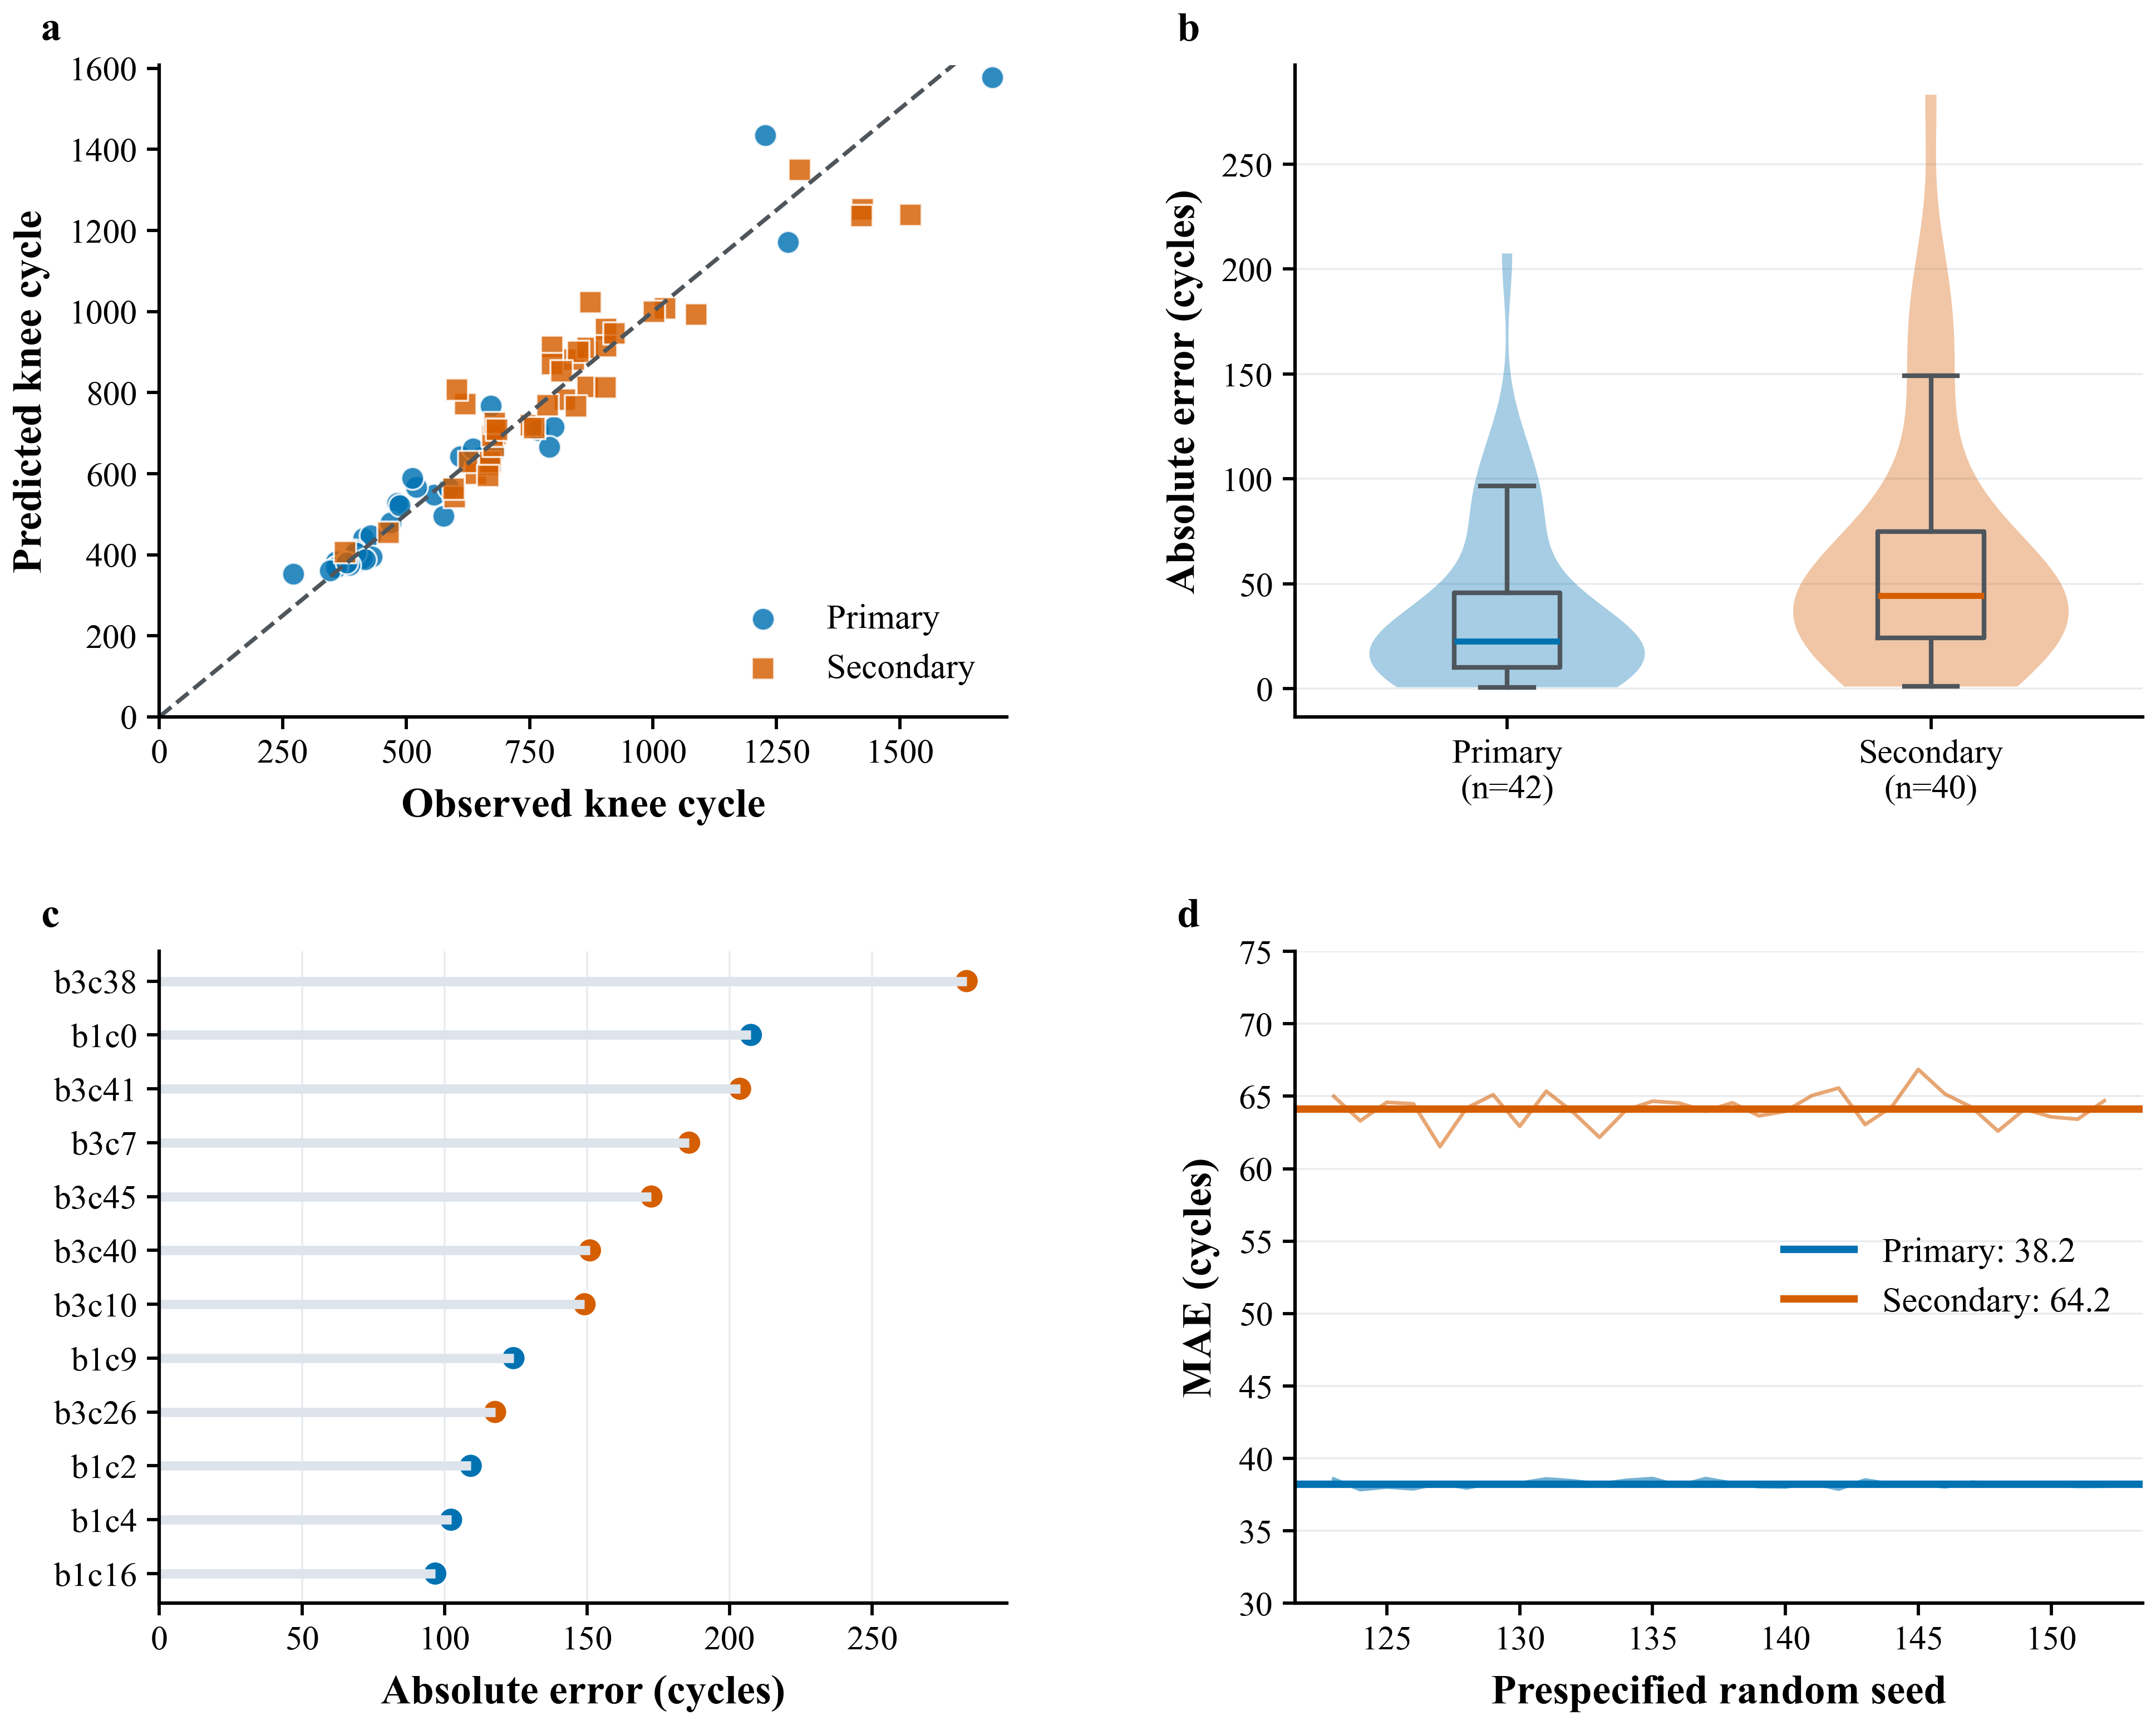
\includegraphics[width=\textwidth]{Figure5.png} 
\caption{Test-cohort performance of the frozen LDQ-ET pipeline. (a) Observed and predicted knee cycles. (b) Absolute-error distributions. (c) The 12 largest cell-level absolute errors. (d) Cohort-level MAE across 30 prespecified ExtraTrees seeds; these values assess algorithmic reproducibility rather than independent experimental replication. Cell identifiers use \texttt{bNcM}, where \texttt{bN} denotes the source batch and \texttt{cM} denotes the cell identifier.} 
\label{fig:external_prediction} 
\end{figure}

As summarized in Table~\ref{tab:heldout_summary}, the frozen model achieved stronger predictive performance on the primary same-batch cohort, with an MAE of 38.23 cycles, an RMSE of 56.87 cycles, and an $R^2$ of 0.957. On the secondary cross-batch cohort, the MAE and RMSE increased to 64.15 and 88.74 cycles, respectively, while $R^2$ decreased to 0.868, indicating a measurable generalization penalty under batch shift. The q90 absolute error also increased from 95.50 to 153.15 cycles, showing that cross-batch transfer enlarged the upper tail of the prediction-error distribution. Nevertheless, the frozen model retained substantial explanatory power in the secondary cohort.

Figure~\ref{fig:external_prediction} provides cell-level context for the cohort-level summaries. Figure~\ref{fig:external_prediction}a shows that predictions in both cohorts broadly follow the identity line, although the primary-test cells are more tightly distributed around it, whereas the secondary cohort exhibits greater dispersion, particularly through the underprediction of several late-knee cells. This contrast is also evident in Figure~\ref{fig:external_prediction}b, where the secondary-cohort absolute-error distribution is shifted toward larger values and has a broader upper tail. Figure~\ref{fig:external_prediction}c shows that seven of the 12 largest cell-level absolute errors, including the largest error, occur in the secondary cohort. Large deviations are therefore present in both cohorts but are more prominent among the secondary cells. Finally, Figure~\ref{fig:external_prediction}d shows that the cohort-level MAEs remain nearly invariant across the 30 prespecified ExtraTrees seeds, at approximately 38.2 cycles for the primary cohort and 64.2 cycles for the secondary cohort. Together, these observations are consistent with the cohort-level performance gap reported in Table~\ref{tab:heldout_summary} and indicate that the gap is not attributable to seed-to-seed variation in model fitting.

The observed pattern is consistent with a distribution shift in the early-cycle descriptors, the knee-cycle labels, or their relationship between the development data and the secondary batch. Because the primary cohort originates from the same batch as the training data, its early-trajectory distribution is more closely aligned with that used to learn the mapping from the Local DeltaQ, raw/SOH, and Global DeltaQ descriptors to the knee cycle. The underprediction of several late-knee cells in the secondary cohort suggests that this mapping transfers less faithfully toward the upper end of the secondary knee-cycle range. However, the observed error patterns alone are insufficient to attribute the cohort-level performance difference to any specific electrochemical mechanism. Distinguishing changes in degradation pathways from differences in measurement conditions, operating histories, or target distributions would require additional batch-level covariates, mechanistic measurements, and evaluation on further independent batches.

\FloatBarrier

\subsection{Matched Regressor Comparison}\label{subsec:regressor_comparison}

% Having established the frozen-pipeline results, we used a matched regressor-family comparison to contextualize the choice of the downstream model. Each candidate used the complete 70-dimensional representation and its prespecified configuration, and repeated training-only cross-validation provided the development comparison. As summarized in Table~\ref{tab:predictor_family}, ExtraTrees achieved the lowest training-CV MAE at 56.36 cycles, ahead of Random Forest at 65.73 cycles, and was therefore mapped to the prespecified 1200-tree final ensemble.

Having established the held-out performance of the frozen LDQ-ET model, we next conducted a matched comparison with alternative regressors to provide a broader performance benchmark. All regressors used the same finalized 70-dimensional representation produced by the fixed Bootstrap-stable selector and were evaluated under the same 150-cycle observation budget, data preprocessing, cohort splits, and prespecified random seeds. The comparison included SVR-RBF as a nonlinear kernel baseline, XGBoost as a gradient-boosted tree model, Random Forest as a bagged tree ensemble, and ExtraTrees as the finalized regressor in LDQ-ET. Table~\ref{tab:predictor_family} summarizes their training-CV, primary-cohort, and secondary-cohort performance.

\begin{table}[!ht]
\caption{Matched comparison of alternative regressors using the complete representation. Values are means across ten prespecified seeds. MAE and q90 are reported in cycles.}
\label{tab:predictor_family}
\centering
\footnotesize
\setlength{\tabcolsep}{2.8pt}
\renewcommand{\arraystretch}{1.16}

\begin{tabularx}{\textwidth}{
@{}
>{\raggedright\arraybackslash}m{0.20\textwidth}
>{\centering\arraybackslash}m{0.13\textwidth}
*{6}{>{\centering\arraybackslash}X}
@{}
}
\toprule
\multicolumn{1}{c}{
  \multirow[c]{2}{*}[-0.5ex]{\makecell[c]{Regressor}}
}
&
\multicolumn{1}{c}{
  \multirow[c]{2}{*}[-0.5ex]{\makecell[c]{Train-CV\\MAE}}
}
& \multicolumn{3}{c}{Primary}
& \multicolumn{3}{c}{Secondary} \\
\cmidrule(lr){3-5}\cmidrule(lr){6-8}
& & MAE & $R^2$ & q90
  & MAE & $R^2$ & q90 \\
\midrule
% Ridge         & 104.86 & 165.84 & -1.440 & 316.24 & 193.62 & -1.900 & 378.80 \\
SVR-RBF       & 70.94  & 75.34  & 0.625  & 146.80 & 159.82 & -0.284 & 328.00 \\
XGBoost       & 63.84  & 61.92  & 0.824  & 137.40 & 115.36 & 0.600  & 238.20 \\
Random Forest & 57.88  & 45.61  & 0.939  & 106.70 & 70.52  & 0.842  & 175.80 \\
ExtraTrees    & 49.76  & 38.23  & 0.957  & 95.50  & 64.15  & 0.868  & 153.15 \\
\bottomrule
\end{tabularx}
\end{table}

Under the matched evaluation, SVR-RBF and XGBoost showed weaker overall performance than the two randomized tree ensembles. The cross-batch limitation was most evident for SVR-RBF, whose secondary-cohort $R^2$ decreased to $-0.284$ and q90 increased to 328.00 cycles. XGBoost improved the secondary-cohort MAE to 115.36 cycles and restored a positive $R^2$ of 0.600, but remained less accurate than the tree ensembles. Random Forest and ExtraTrees produced substantially stronger and more consistent results across the development and held-out evaluations. ExtraTrees achieved the lowest training-CV MAE of 49.76 cycles and retained the most favorable performance on both cohorts, with MAEs of 38.23 and 64.15 cycles on the primary and secondary cohorts, respectively. Its corresponding $R^2$ values remained high at 0.957 and 0.868, while the secondary-cohort q90 was limited to 153.15 cycles. Thus, with the feature representation and evaluation protocol held fixed, LDQ-ET demonstrated the most consistently favorable performance among the tested regressors.

The stronger performance of the two randomized tree ensembles suggests that the finalized 70-dimensional representation contains nonlinear interactions and threshold-dependent relationships that are well suited to tree-based partitioning. Random Forest and ExtraTrees can combine the raw/SOH, Global DeltaQ, and localized descriptors without imposing a single global functional form, which may help accommodate heterogeneous associations across cells. The additional randomization of split thresholds in ExtraTrees may further reduce dependence on particular feature cut points and limit correlation among individual trees, potentially contributing to its more stable same-batch and cross-batch performance.

\FloatBarrier

\subsection{Matched Input Ablation and Early-Observation Performance}
\label{subsec:deep_comparison}

% A matched training-only comparison averaged over ten seeds isolated the contribution of each input block to LDQ-ET performance (Table~\ref{tab:representation_comparison}). Each representation was independently developed on the 41-cell training cohort, with Local DeltaQ blocks reselected within the corresponding training folds. Raw/SOH alone provided a weak baseline, yielding MAEs of 101.30 cycles on the primary-test cohort and 378.98 cycles on the secondary batch. Adding Global DeltaQ produced the first substantial reduction, lowering these errors to 45.99 and 177.40 cycles, respectively. The inclusion of selected Local DeltaQ descriptors then reduced secondary-batch MAE to 90.00 cycles, while the complete representation reached 88.69 cycles. The small difference between these two Local DeltaQ-containing representations indicates that the selected localized descriptors accounted for most of the observed secondary-batch improvement.

To quantify the contribution of each component of the early-cycle representation, we first conducted a matched input comparison under the 150-cycle observation budget. The evaluated configurations progressively incorporated raw capacity/SOH descriptors, Global DeltaQ statistics, and selected Local DeltaQ descriptors, culminating in the complete representation. Except for the training-median reference, each input configuration was developed independently using the same cohort splits, nested-development procedure, ExtraTrees settings, and prespecified random seeds. Any data-dependent feature-selection steps were repeated within the corresponding training splits.

\begin{table}[!ht]
\caption{Matched comparison of independently developed input representations under the 150-cycle observation budget. Values are means across ten prespecified seeds, and MAE is reported in cycles.}
\label{tab:representation_comparison}
\centering
\footnotesize
\setlength{\tabcolsep}{3.5pt}
\renewcommand{\arraystretch}{1.16}
\begin{tabularx}{\textwidth}{@{}>{\centering\arraybackslash}m{0.43\textwidth}>{\centering\arraybackslash}m{0.17\textwidth}>{\centering\arraybackslash}X>{\centering\arraybackslash}X@{}}
\toprule
Input representation & Train-CV & Primary test & Secondary test \\
\midrule
Training median & -- & 168.57 & 400.83 \\
Raw/SOH & 92.76 & 96.84 & 350.12 \\
Raw/SOH + Global DeltaQ & 57.43 & 52.68 & 151.90 \\
Raw/SOH + selected Local DeltaQ & 51.36 & 40.12 & 70.84 \\
Complete representation & 49.76 & 38.23 & 64.15 \\
\bottomrule
\end{tabularx}
\end{table}

Table~\ref{tab:representation_comparison} shows a progressive reduction in prediction error as curve-derived information was added to the Raw/SOH baseline. Global DeltaQ descriptors provided the first substantial improvement, particularly for the secondary test cohort, where the MAE decreased from 350.12 to 151.90 cycles. Adding selected Local DeltaQ descriptors further reduced the secondary-test MAE to 70.84 cycles, indicating that localized discharge-curve changes contributed information beyond whole-curve summaries. The complete representation achieved the lowest MAEs, 38.23 cycles on the primary test and 64.15 cycles on the secondary test, with the smaller gain over the selected-Local-DeltaQ representation suggesting that the retained localized descriptors accounted for most of the improvement.

% \begin{figure}[!ht]
% \centering
% \begin{minipage}[t]{0.48\textwidth}
%   \vspace{0pt}\centering
%   \includegraphics[width=\linewidth]{Figure6a.png}
% \end{minipage}\hfill%
% \begin{minipage}[t]{0.48\textwidth}
%   \vspace{0pt}\centering
%   \includegraphics[width=\linewidth]{Figure6b.png}
% \end{minipage}

% \vspace{0.35em}

% \begin{minipage}[t]{0.48\textwidth}
%   \vspace{0pt}\centering
%   \includegraphics[width=\linewidth]{Figure6c.png}
% \end{minipage}\hfill%
% \begin{minipage}[t]{0.48\textwidth}
%   \vspace{0pt}\centering
%   \includegraphics[width=\linewidth]{Figure6d.png}
% \end{minipage}

% \caption{Early-observation performance on the common $y_i>150$ 41/42/40 cohort. (a) Training-only repeated-CV MAE. (b) Test-cohort MAE with 95\% cell-bootstrap intervals. (c) Changes in MAE relative to the 50-cycle configuration. (d) Cell-level q90 absolute error.}
% \label{fig:budget_learning}
% \end{figure}

\begin{figure}[!ht] 
\centering 
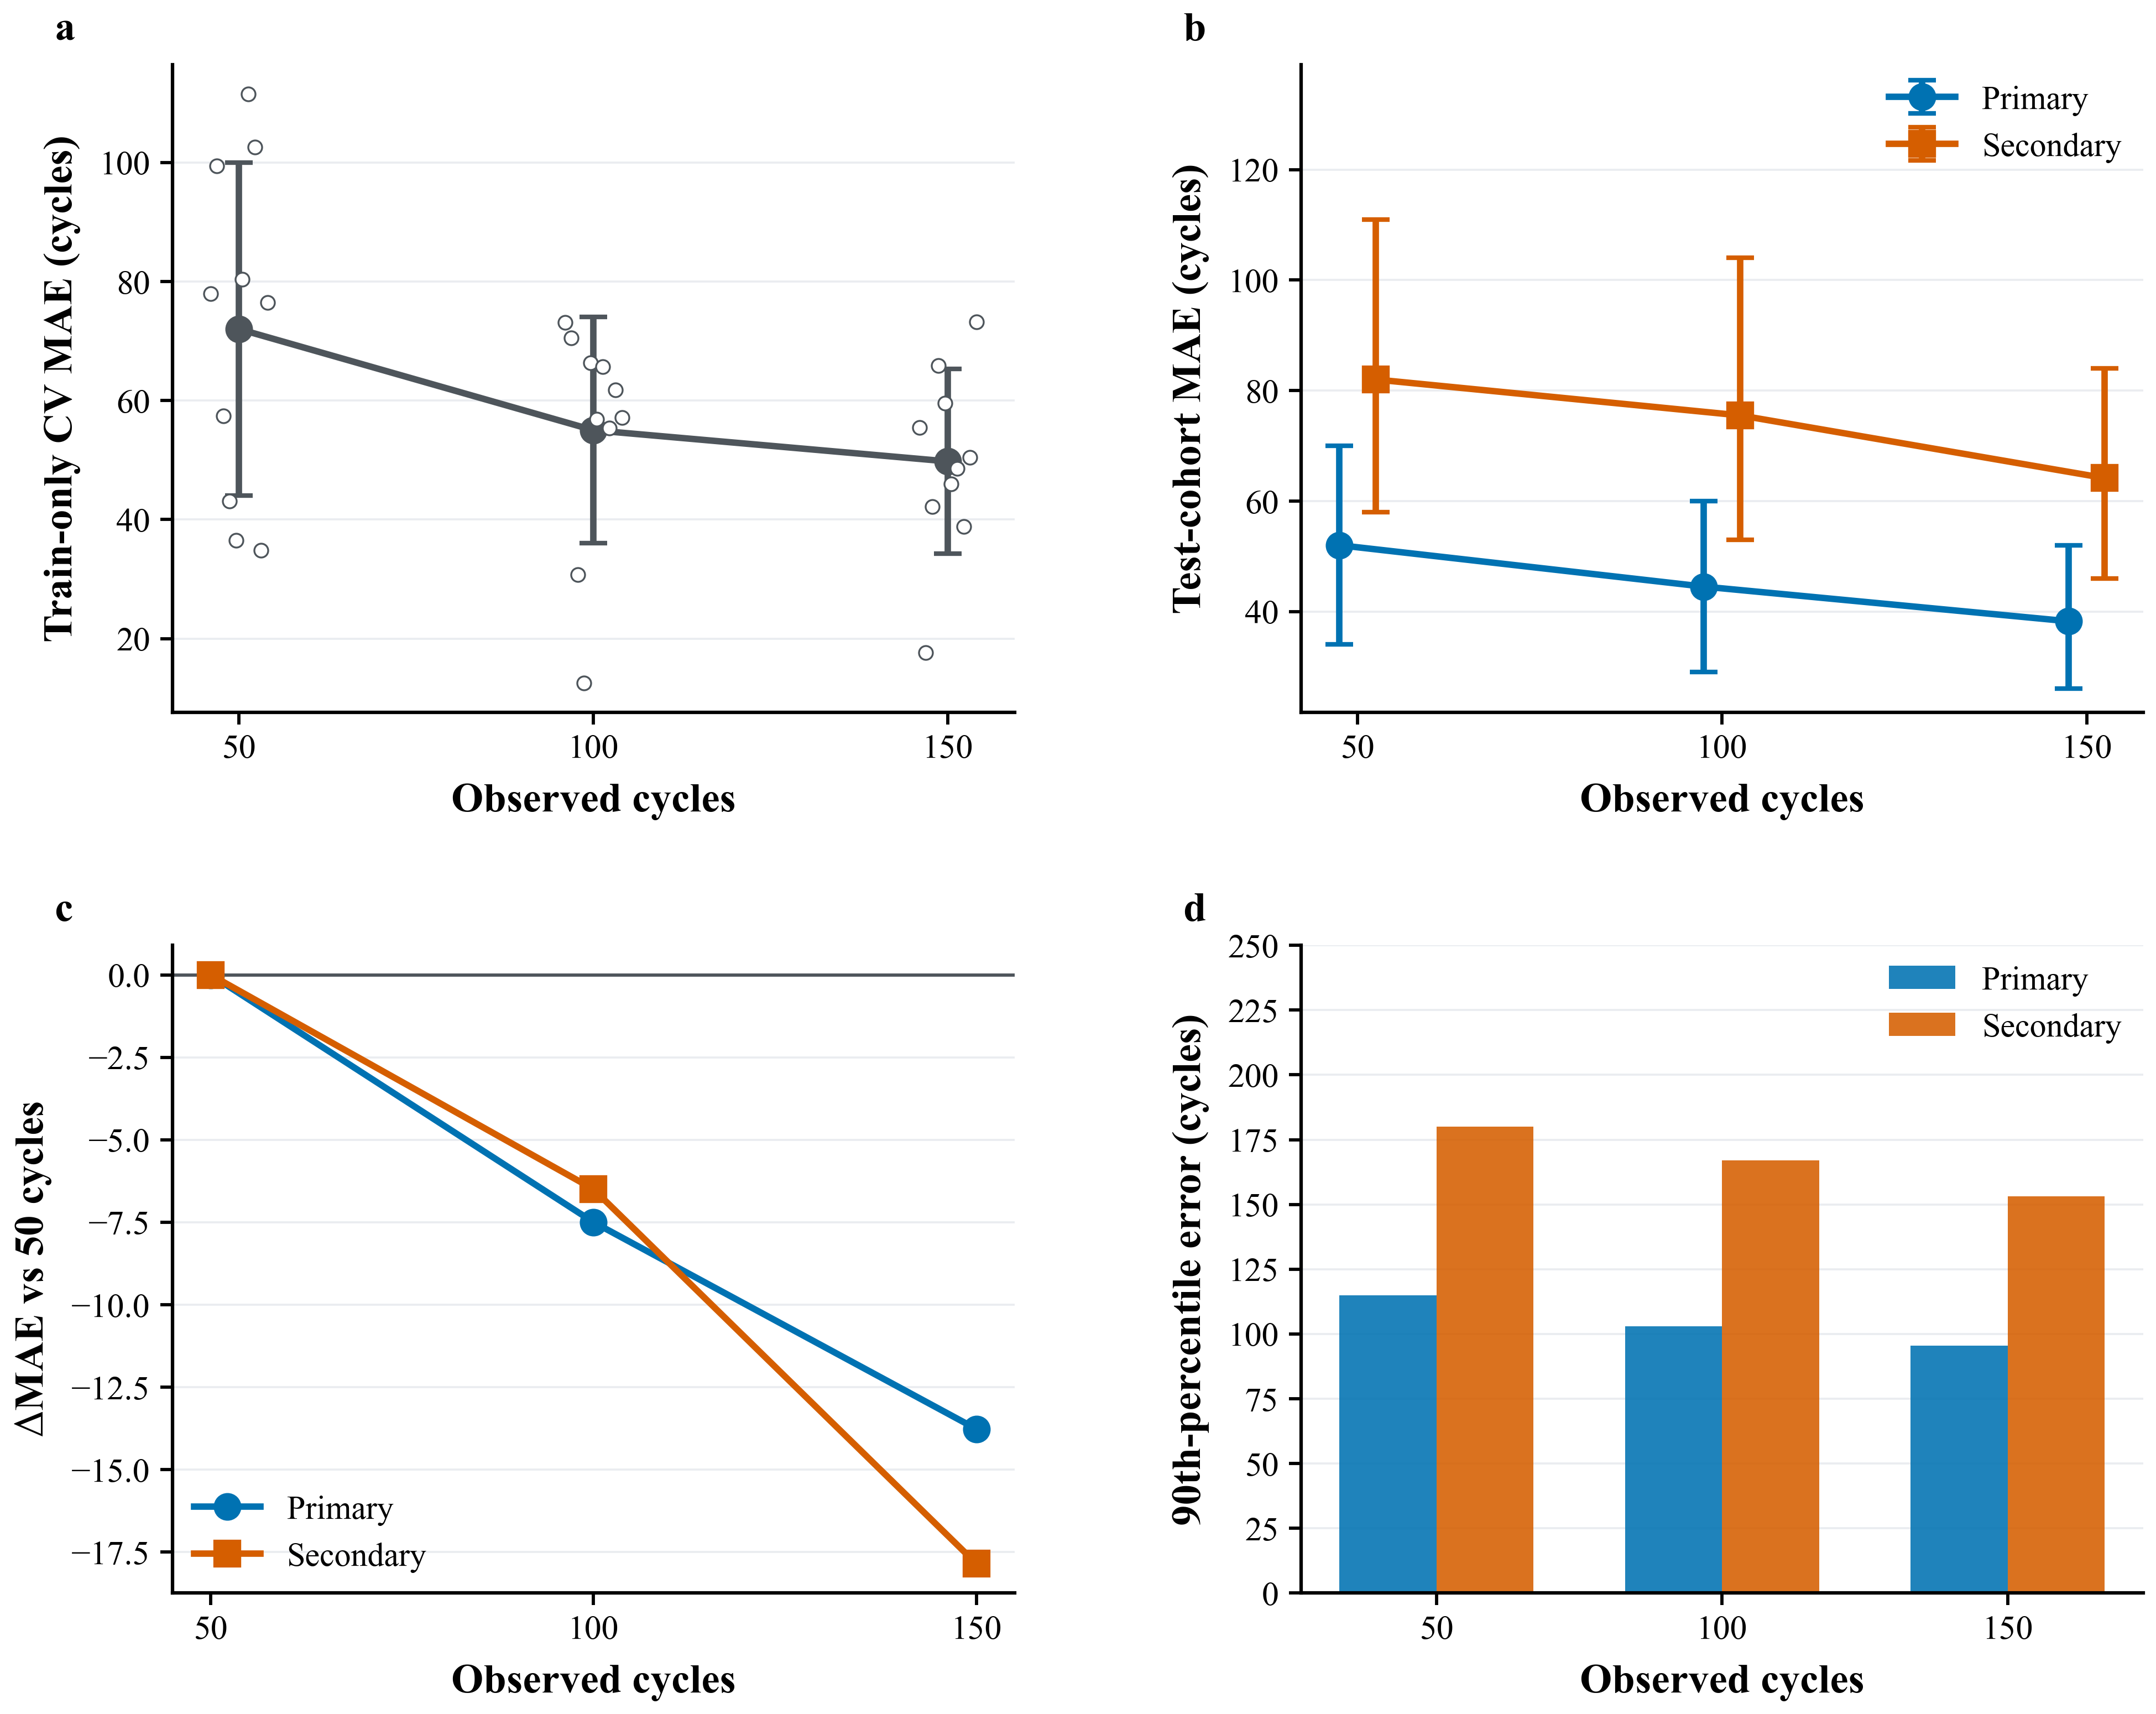
\includegraphics[width=\textwidth]{Figure6.png} 
\caption{Early-observation performance on the common $y_i>150$ 41/42/40 cohort. (a) Training-only repeated-CV MAE. (b) Test-cohort MAE with 95\% cell-bootstrap intervals. (c) Changes in MAE relative to the 50-cycle configuration. (d) Cell-level q90 absolute error.} 
\label{fig:observation_budget} 
\end{figure}

We next assessed the trade-off between prediction earliness and accuracy by comparing observation budgets of 50, 100, and 150 cycles on the common eligibility-controlled 41/42/40 cohorts. At each horizon, the LDQ-ET representation was reconstructed using only measurements available up to that cycle, and all data-dependent selection steps were repeated within the corresponding training splits. Performance was summarized using repeated-CV MAE, held-out MAE with 95\% cell-bootstrap confidence intervals, changes in held-out MAE relative to the 50-cycle configuration, and q90-AE.

Figure~\ref{fig:observation_budget}a indicates that the training-only repeated-CV MAE decreased steadily as the observation window increased, reaching 49.76 cycles at 150 cycles. A similar trend is evident in Figure~\ref{fig:observation_budget}b for the held-out cohorts, where the primary-cohort MAE declined to 38.23 cycles and the secondary-cohort MAE decreased to 64.15 cycles at the longest window. Figure~\ref{fig:observation_budget}c quantifies these improvements relative to the 50-cycle configuration, corresponding to reductions of approximately 14 and 18 cycles, respectively. Figure~\ref{fig:observation_budget}d further illustrates that q90-AE decreased progressively with additional observations, reaching 95.50 cycles for the primary cohort and 153.15 cycles for the secondary cohort at 150 cycles.

Taken together, these results indicate a consistent trade-off between prediction earliness and accuracy. Extending the observation window from 50 to 150 cycles improved both average and upper-tail accuracy in the development evaluation and the two held-out cohorts. Accordingly, the 150-cycle observation budget was adopted for the final LDQ-ET model, as it yielded the lowest repeated-CV MAE and the lowest held-out MAE and q90-AE in both cohorts. Nevertheless, the 50-cycle configuration retained substantial predictive information, suggesting that the framework can support earlier screening when prediction lead time is prioritized over maximum accuracy. 

\FloatBarrier
\subsection{Uncertainty Calibration and Target-Definition Sensitivity}
\label{subsec:robustness}

To further evaluate the robustness of the LDQ-ET framework, we examined prediction-interval calibration under batch shift and the sensitivity of predictive performance to alternative knee-label definitions. Prediction-interval coverage was evaluated on the primary and secondary cohorts, while the piecewise-linear, chord-distance, and degradation-rate-threshold definitions were compared on their common eligible cohort.

\begin{figure}[!ht] 
\centering 
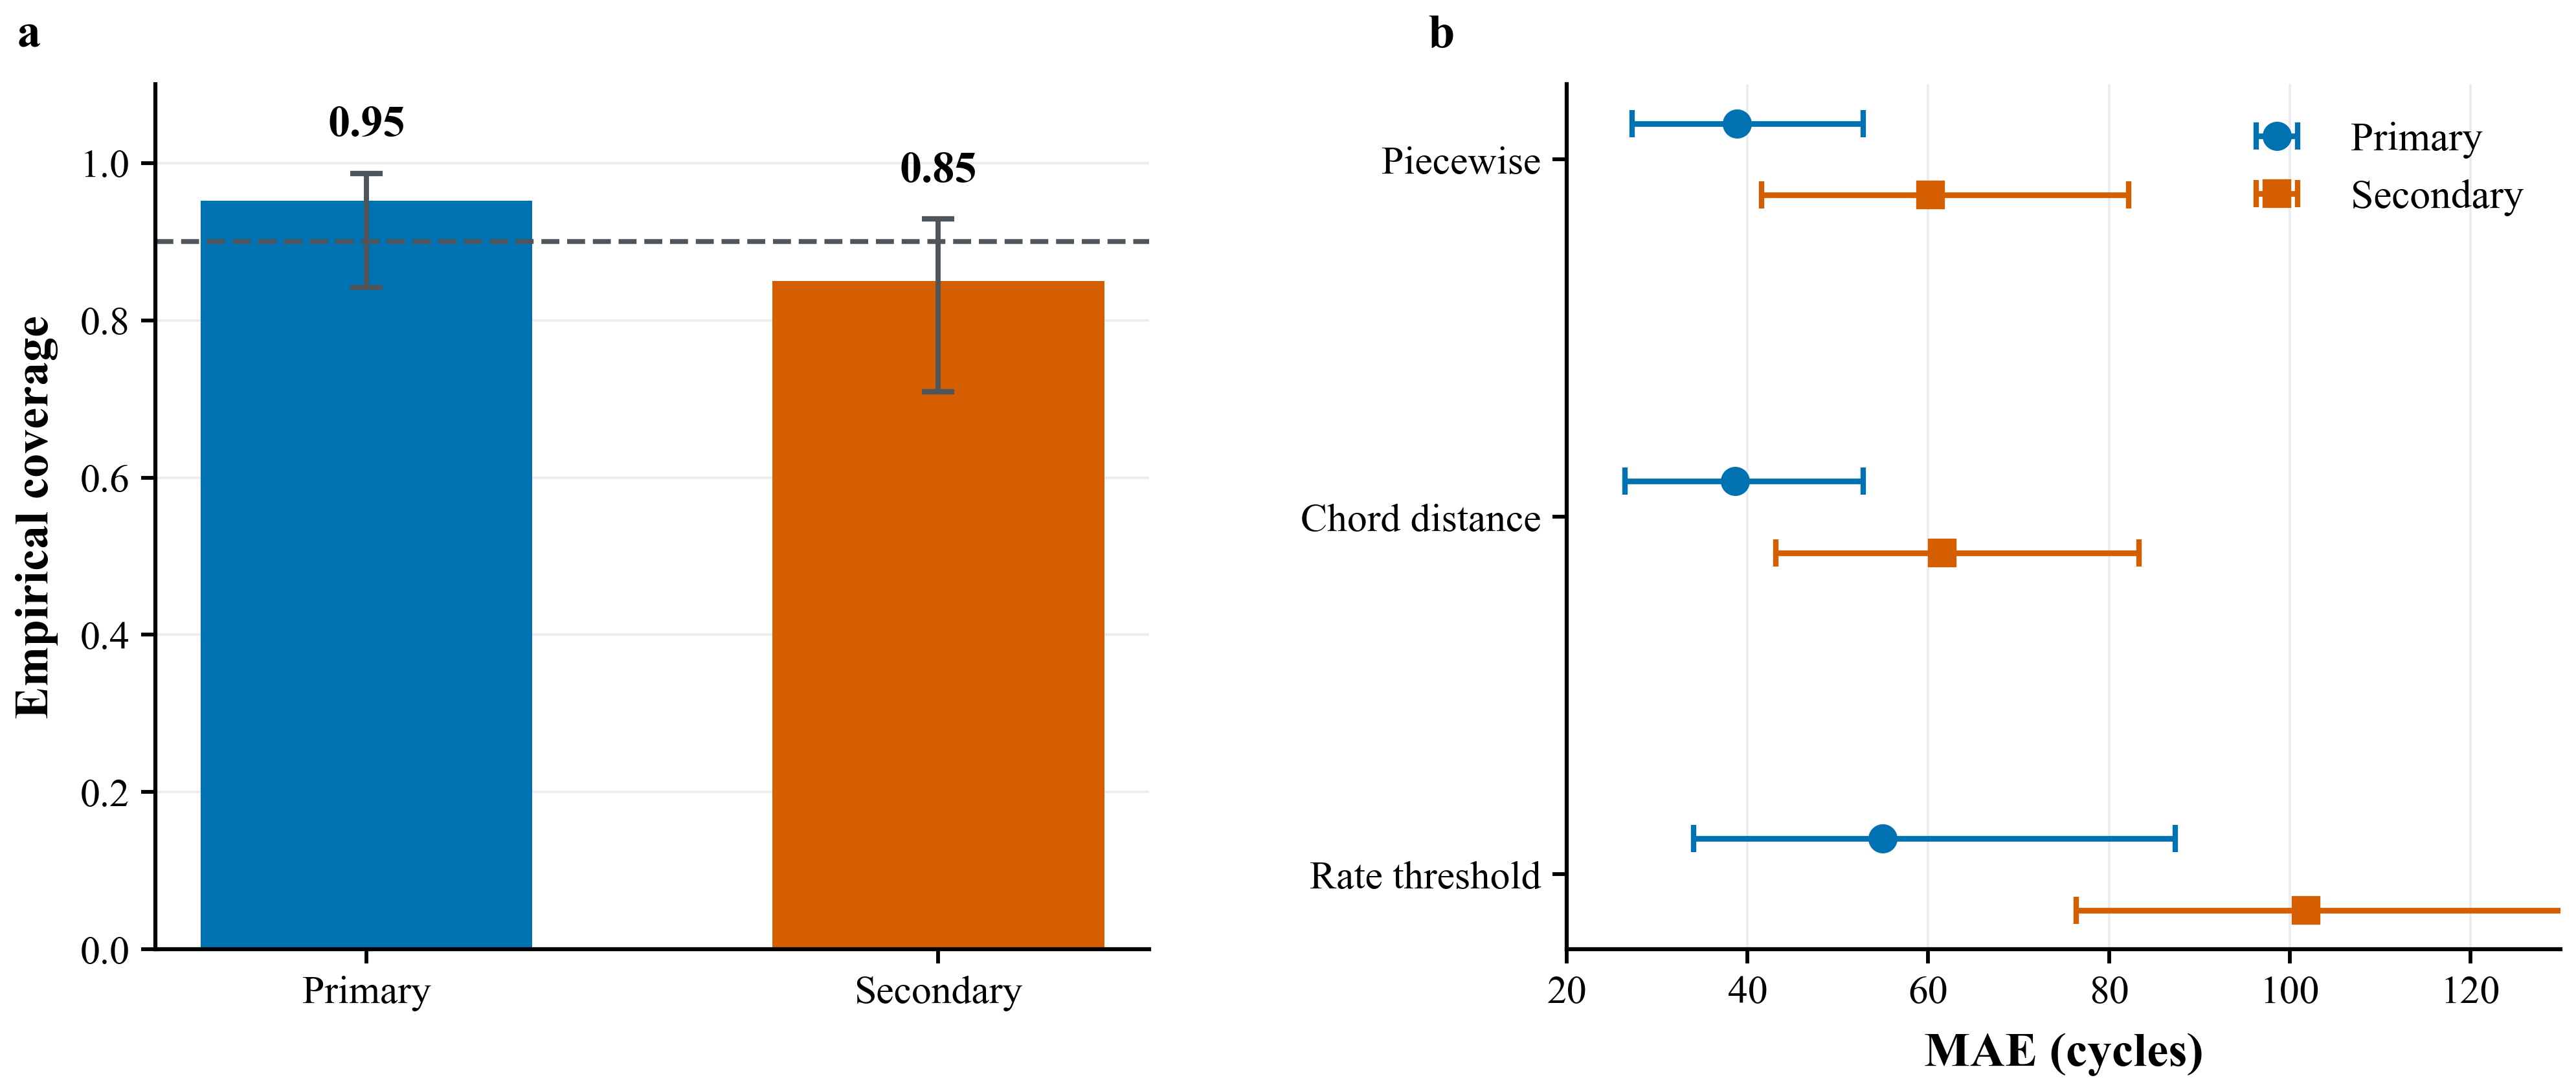
\includegraphics[width=\textwidth]{Figure7.png} 
\caption{Reliability and target-definition sensitivity. (a) Empirical coverage of the training-OOF-calibrated nominal 90\% prediction interval. (b) MAE under three automatic knee-label definitions on their common eligible cohort. Error bars show 95\% cell-bootstrap intervals.} 
\label{fig:reliability_sensitivity} 
\end{figure}

Figure~\ref{fig:reliability_sensitivity}a shows that the training-calibrated prediction interval achieved an empirical coverage of 0.95 on the primary cohort and 0.85 on the secondary cohort. The primary-cohort coverage remained close to the nominal level, whereas the moderate decrease on the secondary cohort indicates that the residual-based calibration transferred less completely under batch shift. This pattern is consistent with the broader secondary-cohort error distribution observed in the point-prediction results. Nevertheless, the interval continued to cover most secondary-cohort cells, indicating that the uncertainty information derived from the training residuals remained informative after cross-batch transfer. The error bars in Figure~\ref{fig:reliability_sensitivity}a denote 95\% Wilson confidence intervals for the empirical coverage estimates.

Figure~\ref{fig:reliability_sensitivity}b compares the held-out MAEs obtained under the three knee-label definitions. The piecewise-linear and chord-distance definitions produced similar errors on both cohorts, with strongly overlapping cell-bootstrap confidence intervals. Their agreement indicates that the predictive results were relatively stable across these two closely related geometric descriptions of the degradation transition. In contrast, the degradation-rate-threshold definition resulted in higher MAEs, with the increase being particularly pronounced on the secondary cohort. This pattern suggests that the degradation-rate-threshold rule defines a more challenging prediction target than the two geometry-based alternatives.

Together, these results show that LDQ-ET is comparatively stable across the two geometry-based knee definitions, whereas the degradation-rate-threshold label defines a more difficult early-prediction target. The lower interval coverage in the secondary cohort further indicates that uncertainty calibration transfers less completely under batch shift. Distribution shift and substantive changes in target construction therefore remain important sources of uncertainty in early knee-cycle prediction.

\FloatBarrier

\section{Conclusion}
\label{sec:conclusion}

This study presented a rigorous, reproducible pipeline for early battery degradation prediction, systematically comparing representation design, regressor selection, observation budgets, and target sensitivity under strict cohort isolation. On the frozen evaluation protocol, the finalized pipeline achieved MAEs of 38.23 cycles on the independent same-batch primary-test cohort and 64.15 cycles on the secondary-batch test cohort. Independently developed representation comparisons confirmed that inputs incorporating selected Local $\Delta Q$ descriptors retained substantially lower cross-batch error than Raw/SOH or Raw/SOH + Global $\Delta Q$ alternatives.

Across the evaluated regressors, ExtraTrees consistently provided the lowest development, primary-test, and secondary-batch errors. Increasing the observation budget from 50 to 150 cycles progressively improved point accuracy and reduced tail errors ($q_{90}$) across cohorts, reaching optimal performance at the 150-cycle setting. Sensitivity analyses on the degradation-rate-threshold further emphasized that predictive accuracy remains conditional on target definitions.

Beyond the performance gains summarized above, the results also identify two practical limitations that motivate further development. First, performance degraded under secondary-batch evaluation, indicating that the current feature representation remains sensitive to batch-to-batch manufacturing and testing shifts. Second, the framework relies on fixed early-cycle observation budgets of 50--150 cycles, which may constrain real-time applicability when continuous early-life data are incomplete. Future work will therefore investigate domain-adaptation methods to mitigate cross-batch distribution shifts and develop dynamic observation models that remain effective with incomplete operational data.

\backmatter

\section*{Declarations}

\noindent\textbf{Authors' contributions} Chang Liu contributed to Conceptualization, Investigation, Methodology, Software, Validation, Visualization, and Writing---original draft. Congyan Chen contributed to Formal analysis, Funding acquisition, Project administration, Supervision, Validation, and Writing---review and editing.

\noindent\textbf{Funding} This work was supported by the Guangdong Basic and Applied Basic Research Foundation (Grant No.~2024A1515011962).

\noindent\textbf{Data availability} Data will be made available on request.

\noindent\textbf{Competing interests} The authors declare no competing interests.

\setlength{\bibsep}{0pt}
\bibliography{references}

\end{document}
